\documentclass[11pt,a4paper]{article}

\usepackage[utf8]{inputenc}
\usepackage[T1]{fontenc}
\usepackage[spanish,es-tabla]{babel}
\usepackage{lmodern}
\usepackage[margin=2.5cm]{geometry}
\usepackage{booktabs}
\usepackage{array}
\usepackage{makecell}
\usepackage{graphicx}
\usepackage{float}
\usepackage{caption}
\usepackage{subcaption}
\usepackage{enumitem}
\usepackage{amsmath}
\usepackage{setspace}
\usepackage[hidelinks]{hyperref}
\usepackage[round,authoryear]{natbib}

\graphicspath{{../figuras/}{figuras/}}
\setstretch{1.1}
\setlength{\parskip}{0.7em}
\setlength{\parindent}{0pt}
\setlength{\bibhang}{0pt}
\setlength{\bibsep}{5pt}
\renewcommand{\refname}{Referencias}
\setcitestyle{aysep={,}}
\captionsetup{font=small,labelfont=bf}
\newcolumntype{P}[1]{>{\raggedright\arraybackslash}p{#1}}

\newcommand{\mcbaselinelongitud}{0{,}724}
\newcommand{\rcbaselinelongitud}{0{,}559}
\newcommand{\rwbaselinelongitud}{0{,}865}
\newcommand{\mcridgebase}{0{,}592}
\newcommand{\rcridgebase}{0{,}495}
\newcommand{\rwridgebase}{0{,}674}
\newcommand{\mcridgeenriquecido}{0{,}567}
\newcommand{\rcridgeenriquecido}{0{,}466}
\newcommand{\rwridgeenriquecido}{0{,}651}
\newcommand{\mclgbmbase}{0{,}546}
\newcommand{\rclgbmbase}{0{,}466}
\newcommand{\rwlgbmbase}{0{,}615}
\newcommand{\mclgbmenriquecido}{0{,}524}
\newcommand{\rclgbmenriquecido}{0{,}448}
\newcommand{\rwlgbmenriquecido}{0{,}587}
\newcommand{\mcdebertabase}{0{,}608}
\newcommand{\rcdebertabase}{0{,}484}
\newcommand{\rwdebertabase}{0{,}737}
\newcommand{\mcdebertasmall}{0{,}617}
\newcommand{\rcdebertasmall}{0{,}481}
\newcommand{\rwdebertasmall}{0{,}754}
\newcommand{\mcensamble}{0{,}518}
\newcommand{\rcensamble}{0{,}433}
\newcommand{\rwensamble}{0{,}588}
\newcommand{\mcensamblerasgos}{0{,}545}
\newcommand{\rcensamblerasgos}{0{,}460}
\newcommand{\rwensamblerasgos}{0{,}616}


\begin{document}

%%%%%%%%%%%%%%%%%%%%%%%%%%%% PORTADA %%%%%%%%%%%%%%%%%%%%%%%%%%%%
\begin{titlepage}
\centering
{\large Universidad del Valle de Guatemala\\
Facultad de Ingeniería\\
Departamento de Ciencias de la Computación\\
CC3084 --- Data Science\\
Semestre II --- 2026\par}

\vspace{2.2cm}

{\LARGE Proyecto 2 --- Informe final\par}
\vspace{0.8cm}
{\large Reto 12: CommonLit --- Evaluar resúmenes de estudiantes\par}
\vspace{0.3cm}
{\normalsize Tema: Procesamiento del Lenguaje Natural\par}
\vspace{0.3cm}
{\small \url{https://www.kaggle.com/competitions/commonlit-evaluate-student-summaries/overview}\par}

\vspace{1.5cm}
{\Large Grupo 6\par}
\vspace{0.4cm}
Jose López --- 23773\\
Hugo Barillas --- 23306\\
Luis Palacios --- 23933\\
Roberto Nájera --- 23781

\vfill
Guatemala, 19 de octubre de 2026
\end{titlepage}

\tableofcontents
\newpage
%%%%%%%%%%%%%%%%%%%%%%%%%%%% 1. INTRODUCCIÓN %%%%%%%%%%%%%%%%%%%%%%%%%%%%
\section{Introducción}

Escribir un buen resumen ayuda a los estudiantes a comprender lo que leen y a mejorar su escritura, pero calificar resúmenes a mano consume tiempo, la nota cambia según quién califica y la retroalimentación llega tarde. Por eso los profesores asignan pocos ejercicios de resumen y los estudiantes practican poco. CommonLit y otras organizaciones publicaron un conjunto de 7\,165 resúmenes escritos por estudiantes de tercero a doceavo grado sobre cuatro textos, cada uno con dos notas puestas por expertos: \emph{content}, que mide qué tan bien el resumen recoge las ideas principales del texto original, y \emph{wording}, que mide la claridad y la calidad de la redacción.

El problema que aborda este proyecto es predecir esas dos notas de forma automática usando únicamente el texto del resumen y el texto fuente, de manera que el modelo también funcione con textos fuente que no vio durante el entrenamiento. La métrica oficial de la competencia es el MCRMSE, el promedio de la raíz del error cuadrático medio de las dos notas.

Este informe reúne todo el trabajo del proyecto. Primero se plantean los objetivos y se presenta el marco teórico, que incluye una revisión bibliográfica de los algoritmos usados en la evaluación automática de escritura. Luego se explica la metodología, en particular la forma de validación, que deja un texto fuente completo fuera en cada iteración. Después se presentan los datos, su limpieza y su análisis exploratorio, el ajuste y la comparación de los modelos, y la aplicación construida para probarlos. El informe cierra con las conclusiones.

%%%%%%%%%%%%%%%%%%%%%%%%%%%% 2. OBJETIVOS %%%%%%%%%%%%%%%%%%%%%%%%%%%%
\section{Objetivos}

\textbf{Objetivo general.} Construir y comparar modelos de aprendizaje automático que predigan las notas \emph{content} y \emph{wording} de resúmenes de estudiantes y que generalicen a textos fuente nuevos, y ponerlos a disposición de un usuario mediante una aplicación interactiva.

\textbf{Objetivos específicos.}
\begin{enumerate}[nosep]
\item Describir la estructura, la calidad y las características de los datos, y registrar la limpieza y el preprocesamiento aplicados.
\item Identificar con estadística y gráficos qué características del texto se relacionan con cada nota.
\item Entrenar varios modelos de familias distintas (regresión regularizada, gradient boosting, modelo de lenguaje preentrenado y combinación de modelos) y ajustar sus hiperparámetros sin filtrar información del texto que se evalúa.
\item Comparar los modelos con el MCRMSE, por texto fuente, por longitud del resumen y por tiempo de cómputo, y decidir cuál usar.
\item Construir una aplicación en la que se puedan ingresar resúmenes nuevos, ver el resultado de cada algoritmo por separado o de todos, y explorar los datos y el rendimiento mediante gráficas interactivas.
\end{enumerate}
%%%%%%%%%%%%%%%%%%%%%%%%%%%% 3. MARCO TEÓRICO %%%%%%%%%%%%%%%%%%%%%%%%%%%%
\section{Marco teórico}

\subsection{Procesamiento del lenguaje natural}

El procesamiento del lenguaje natural (PLN) es el área de la inteligencia artificial y la lingüística computacional que desarrolla métodos para que una computadora lea, interprete y genere lenguaje humano \citep{hirschberg2015}. Sus tareas van desde etiquetar palabras y analizar la estructura de las oraciones hasta clasificar documentos, traducir y resumir. La evaluación automática de escritura es una aplicación de PLN a la educación: dado un texto escrito por un estudiante, el sistema estima una nota que se compara con la de calificadores humanos \citep{hussein2019,ramesh2022}. En este proyecto la tarea es de \emph{regresión}, porque las dos notas son numéricas y continuas, y es \emph{multi-salida}, porque se predicen dos notas a la vez.

\subsection{Actividades de preprocesamiento}

Un modelo no lee texto crudo, y las decisiones de preprocesamiento cambian su desempeño \citep{uysal2014}. Las actividades más comunes son las siguientes.
\begin{itemize}[nosep]
\item \textbf{Limpieza y normalización}: unificar espacios y saltos de línea y quitar caracteres de control. Opcionalmente se pasa a minúsculas y se eliminan signos.
\item \textbf{Tokenización}: dividir el texto en unidades, que pueden ser palabras, oraciones, caracteres o subpalabras. Los modelos Transformer usan subpalabras para representar cualquier palabra, incluso las que tienen errores de ortografía.
\item \textbf{Palabras vacías}: quitar o contar las palabras muy frecuentes y poco informativas (por ejemplo \emph{the} o \emph{of}).
\item \textbf{Lematización y derivación}: reducir las palabras a su raíz. No se usa en este proyecto porque se quiere conservar la forma exacta en que escribió el estudiante.
\item \textbf{Representación numérica}: convertir el texto en números mediante rasgos diseñados a mano, bolsa de palabras ponderada (TF-IDF), semántica latente o vectores aprendidos por una red neuronal.
\end{itemize}
En la evaluación de escritura \textbf{no} se debe borrar la puntuación ni las mayúsculas, porque son señales de calidad de redacción. Por eso la limpieza de este proyecto solo normaliza espacios y caracteres de control.

\subsection{Rasgos del texto}

Los sistemas clásicos de puntuación calculan rasgos interpretables \citep{attali2006}. Los que se usan aquí son:
\begin{itemize}[nosep]
\item \textbf{Tamaño}: caracteres, palabras, oraciones, comas y longitud media de palabra y de oración.
\item \textbf{Diversidad léxica}: la razón entre palabras distintas y palabras totales (\emph{type-token ratio}, TTR) baja de forma natural cuando el texto crece, así que mide tamaño y no riqueza de vocabulario \citep{mccarthy2010}. Por eso se usa también el índice de Guiraud, $G = U/\sqrt{N}$, con $U$ palabras distintas y $N$ palabras totales, que compensa en parte ese efecto.
\item \textbf{Legibilidad}: fórmulas que combinan la longitud de las oraciones y de las palabras. La facilidad de lectura de Flesch es $206{,}835 - 1{,}015\,(N/S) - 84{,}6\,(Sil/N)$, con $S$ oraciones y $Sil$ sílabas \citep{flesch1948}. También se calculan el grado de Flesch-Kincaid, el índice Gunning Fog y el índice ARI.
\item \textbf{Solapamiento con el texto fuente}: proporción de palabras, bigramas y trigramas del resumen que aparecen en el texto original. Distingue parafrasear de copiar y pegar.
\item \textbf{Ortografía}: proporción de palabras que un corrector no reconoce.
\item \textbf{Semántica y cobertura}: se representan el resumen y el texto fuente con TF-IDF \citep{salton1988}, que pondera más las palabras que distinguen a un documento, y con análisis semántico latente (LSA), que reduce esa matriz a pocas dimensiones mediante descomposición en valores singulares \citep{landauer1998}. La similitud coseno entre el resumen y la fuente aproxima la cobertura de contenido, que es la idea de Summary Street \citep{kintsch2000}. Además se mide la similitud del resumen con cada oración de la fuente para saber cuántas ideas del original toca.
\end{itemize}

\subsection{Algoritmos de aprendizaje automático}

\textbf{Regresión Ridge.} Es una regresión lineal con penalización L2 sobre los coeficientes, $\min_\beta \lVert y - X\beta\rVert^2 + \alpha\lVert\beta\rVert^2$ \citep{hoerl1970}. La penalización estabiliza los coeficientes cuando hay rasgos correlacionados, como la cantidad de palabras y de caracteres. Es interpretable y rápida.

\textbf{Gradient boosting.} Construye un conjunto de árboles de decisión pequeños, cada uno entrenado para corregir los errores de los anteriores \citep{friedman2001}. LightGBM \citep{ke2017} acelera el método agrupando los valores de cada rasgo en intervalos y haciendo crecer los árboles hoja por hoja. Captura relaciones no lineales e interacciones, y es competitivo con las redes profundas en datos tabulares \citep{shwartz2022}.

\textbf{Transformers y DeBERTa.} Un Transformer procesa todas las palabras de un texto a la vez mediante atención, que calcula cuánto debe influir cada palabra en la representación de las demás. BERT \citep{devlin2019} se preentrena con grandes cantidades de texto y luego se ajusta a una tarea concreta. DeBERTa \citep{he2021} codifica por separado el contenido y la posición de cada palabra, y DeBERTaV3 \citep{he2023} cambia el objetivo de preentrenamiento por la detección de palabras reemplazadas. Para regresión se añade sobre el modelo una capa lineal que produce las notas. El ajuste fino con una cabeza de dos salidas permite predecir \emph{content} y \emph{wording} con una sola red.

\textbf{Combinación de modelos (stacking).} Un metamodelo aprende a ponderar las predicciones de varios modelos base \citep{wolpert1992}. Para que no haya fuga de información, las predicciones que recibe deben ser fuera de muestra.


\subsection{Revisión bibliográfica de algoritmos para evaluar escritura}

La revisión del documento de avances se resume a continuación; la selección de modelos que se derivó de ella está en la sección~\ref{sec:metodologia}.

\subsubsection{Panorama general de la evaluación automática de textos}

La evaluación automática de escritura es un área consolidada. \citet{hussein2019} y \citet{ramesh2022} presentan revisiones de la literatura que muestran una evolución clara, desde sistemas basados en rasgos lingüísticos diseñados a mano, hacia modelos estadísticos de aprendizaje automático y, más recientemente, hacia redes neuronales y modelos de lenguaje preentrenados. \citet{uto2021} revisa de forma específica los modelos neuronales y clasifica la tarea de puntuación en cuatro tipos. \citet{williamson2012} propone un marco para decidir si un sistema de puntuación automática es adecuado, que considera el ajuste con el propósito de la evaluación, la concordancia con calificadores humanos, la asociación con medidas independientes, la generalización entre tareas y los efectos sobre subgrupos. Este marco es relevante para el proyecto porque un modelo que solo cuenta palabras acertaría bastante, pero no evaluaría contenido ni redacción, y porque la generalización a textos nuevos es el reto central.

\subsubsection{Sistemas clásicos basados en rasgos y regresión}

Los sistemas comerciales clásicos combinan rasgos lingüísticos con un modelo lineal. E-rater V.2 \citep{attali2006} usa un conjunto pequeño de rasgos interpretables y un único modelo de puntuación que sirve para todos los textos de una evaluación, lo que lo acerca al problema de generalizar entre textos fuente. Su ventaja es que cada rasgo se puede explicar y traducir en retroalimentación.

Otra línea son las herramientas de análisis lingüístico automático que producen cientos de índices. TAACO calcula índices de cohesión local y global, y se reporta que los índices globales predicen juicios de expertos sobre la coherencia y la calidad de los ensayos \citep{crossley2016}. TAALES calcula índices de sofisticación léxica como frecuencia de palabras, asociación entre n-gramas y distintividad contextual, y sus índices explican una parte importante de la variación en las notas de dominio léxico \citep{kyle2018}. Estas familias coinciden con las del marco teórico del análisis exploratorio, que incluye diversidad léxica, cohesión y solapamiento.

Sobre estos rasgos se han aplicado la regresión regularizada \citep{hoerl1970}, las máquinas de vectores de soporte para regresión \citep{cortes1995,smola2004}, los bosques aleatorios \citep{breiman2001} y el gradient boosting \citep{friedman2001}, con implementaciones modernas como XGBoost \citep{chen2016} y LightGBM \citep{ke2017}. El esquema de ponderación TF-IDF \citep{salton1988} sigue siendo la representación base para texto cuando no se usan embeddings.

\subsubsection{Semántica latente y evaluación de resúmenes}

Para resúmenes en particular, la línea más influyente es el análisis semántico latente, que representa los textos en un espacio de baja dimensión y permite medir su similitud semántica \citep{landauer1998}. Sobre esta idea se construyó Summary Street, un sistema que compara el resumen del estudiante con el texto original, estima si cubre el contenido importante y le indica qué información de la fuente falta \citep{kintsch2000}. \citet{wade2004} describen su uso con estudiantes de sexto grado para resúmenes de entre 100 y 250 palabras, y \citet{franzke2005} presentan el sistema como apoyo a la comprensión y la escritura. Esto respalda la idea de que la cobertura de contenido, es decir la nota content, se puede aproximar con la similitud semántica entre el resumen y la fuente.

La similitud entre un resumen y su fuente también se puede medir con embeddings de oraciones. Sentence-BERT \citep{reimers2019} usa redes siamesas sobre BERT para producir vectores que se comparan con similitud coseno. Por su parte, fastText \citep{bojanowski2017} representa cada palabra con los n-gramas de sus caracteres y puede generar vectores para palabras que no vio en el entrenamiento, lo que da robustez ante los errores de ortografía frecuentes en textos de estudiantes.

\subsubsection{Redes neuronales para puntuación de ensayos}

Con el aumento de datos, los modelos neuronales empezaron a sustituir la ingeniería de rasgos. \citet{taghipour2016} entrenan redes recurrentes LSTM \citep{hochreiter1997} que aprenden la relación entre el ensayo y su nota sin rasgos manuales y superan una línea base fuerte en 5,6 por ciento de kappa ponderado cuadrático. \citet{kumar2020} usan perceptrones multicapa para predecir notas holísticas y por rúbrica, y emplean valores SHAP para explicar las predicciones, con lo que responden a la crítica de que las redes son cajas negras. \citet{uto2021} presenta en detalle la arquitectura de los modelos neuronales de puntuación y señala que este enfoque evita la ingeniería de rasgos.

\subsubsection{Modelos de lenguaje preentrenados}

Los modelos de tipo Transformer representan el estado del arte actual. BERT \citep{devlin2019} introdujo el preentrenamiento bidireccional y el ajuste fino para tareas específicas. \citet{xue2021} ajustan BERT con aprendizaje multitarea y un esquema jerárquico para textos largos, a fin de predecir varias dimensiones de calidad a la vez, y reportan una mejora de 4,5 por ciento en el kappa ponderado cuadrático sobre una línea base fuerte en el conjunto ASAP. \citet{ludwig2021} comparan modelos Transformer con una regresión logística sobre bolsa de palabras para calificar respuestas escritas por correo electrónico y encuentran que los Transformers la superan sin ajuste de hiperparámetros.

DeBERTa \citep{he2021} mejora a BERT mediante una atención desacoplada, que codifica por separado el contenido y la posición de cada palabra, y un decodificador de máscara mejorado. DeBERTaV3 \citep{he2023} reemplaza el objetivo de enmascaramiento por la detección de tokens reemplazados, al estilo ELECTRA, y usa una compartición de embeddings desacoplada por gradiente. Estos modelos se ofrecen en distintos tamaños, como small, base y large, con un costo computacional creciente.

Los modelos de lenguaje generativos también se han explorado como evaluadores. \citet{mizumoto2023} reportan una correlación entre las puntuaciones de un modelo generativo, usado sin entrenamiento específico, y el nivel de ensayos de TOEFL.

\subsubsection{Calificación de respuestas cortas}

La calificación automática de respuestas cortas está cerca del problema de los resúmenes, porque la respuesta del estudiante se compara con una referencia. \citet{burrows2015} organizan los trabajos de esta área en eras, que van del mapeo de conceptos y la extracción de información a los métodos basados en corpus, el aprendizaje automático y la evaluación, y reúnen más de ochenta trabajos.

\subsubsection{Datos tabulares, ensambles y combinación de modelos}

Un hallazgo repetido es que los modelos de árboles potenciados siguen siendo competitivos frente a las redes profundas en datos tabulares, y que combinar ambos da los mejores resultados. \citet{shwartz2022} comparan modelos profundos recientes con XGBoost sobre varios conjuntos de datos y encuentran que XGBoost es superior y requiere menos ajuste, mientras que un ensamble de modelos profundos con XGBoost suele ser la mejor opción. La generalización apilada \citep{wolpert1992} formaliza esta combinación, ya que un metamodelo aprende a ponderar las predicciones de modelos base.

\subsubsection{Síntesis comparativa}

La tabla \ref{tab:familias} resume las familias revisadas, sus fortalezas y sus limitaciones frente al problema de este proyecto.

\begin{table}[ht]
\centering
\footnotesize
\caption{Comparación de familias de algoritmos revisadas.}
\label{tab:familias}
\begin{tabular}{P{2.7cm}P{3.3cm}P{3.3cm}P{3.3cm}}
\toprule
Familia & Referencias & Fortalezas & Limitaciones \\
\midrule
Regresión lineal o regularizada sobre rasgos &
\citet{attali2006}; \citet{hoerl1970} &
Interpretable, rápida y buena línea base. &
Capacidad limitada y no captura significado. \\
\addlinespace
Árboles y boosting sobre rasgos &
\citet{breiman2001}; \citet{friedman2001}; \citet{chen2016}; \citet{ke2017}; \citet{shwartz2022} &
Captura no linealidades e interacciones, necesita poco ajuste. &
Depende de la calidad de los rasgos y puede reducirse a contar palabras. \\
\addlinespace
Similitud semántica con LSA o embeddings &
\citet{landauer1998}; \citet{kintsch2000}; \citet{reimers2019}; \citet{bojanowski2017} &
Mide la cobertura de contenido frente a la fuente. &
Poco sensible a la redacción y requiere el texto fuente. \\
\addlinespace
Redes recurrentes y perceptrones &
\citet{taghipour2016}; \citet{hochreiter1997}; \citet{kumar2020} &
Aprenden representaciones sin rasgos manuales. &
Necesitan muchos datos variados y generalizan peor a textos nuevos. \\
\addlinespace
Transformers ajustados &
\citet{devlin2019}; \citet{he2021}; \citet{he2023}; \citet{xue2021}; \citet{ludwig2021} &
Significado en contexto y varias salidas a la vez. &
Costo computacional y límite de longitud de entrada. \\
\addlinespace
Modelos generativos sin entrenar &
\citet{mizumoto2023} &
No requieren datos etiquetados. &
Costo y poca reproducibilidad. \\
\addlinespace
Ensambles y stacking &
\citet{wolpert1992}; \citet{shwartz2022} &
Combinan señales complementarias y reducen la varianza. &
Mayor complejidad y riesgo de fuga si no se valida bien. \\
\bottomrule
\end{tabular}
\end{table}


\subsection{Métrica y validación}

La métrica de la competencia es el \textbf{MCRMSE} (\emph{mean columnwise root mean squared error}):
\[
\mathrm{MCRMSE}=\frac{1}{2}\sum_{j\in\{\text{content},\text{wording}\}}\sqrt{\frac{1}{n}\sum_{i=1}^{n}\left(y_{ij}-\hat y_{ij}\right)^2}.
\]
Es un error en las mismas unidades que las notas, así que menor es mejor. Como las notas están casi estandarizadas (desviación cercana a 1), predecir siempre la media da un MCRMSE cercano a 1.

Cuando los datos están agrupados, como aquí, donde muchos resúmenes comparten el mismo texto fuente, una validación cruzada con particiones al azar mezcla resúmenes del mismo texto en entrenamiento y prueba y subestima el error que se tendrá con textos nuevos. La validación debe separar por grupo \citep{roberts2017}. Aquí el grupo es el texto fuente y se deja un texto completo fuera en cada iteración (\emph{Leave-One-Prompt-Out}).

%%%%%%%%%%%%%%%%%%%%%%%%%%%% 4. METODOLOGÍA %%%%%%%%%%%%%%%%%%%%%%%%%%%%
\section{Metodología}\label{sec:metodologia}

\subsection{Pasos seguidos}

\begin{enumerate}[nosep]
\item \textbf{Análisis exploratorio} de las dos tablas de entrenamiento, con 21 características derivadas del texto y su relación con las notas (entrega anterior).
\item \textbf{Revisión bibliográfica} de algoritmos para evaluar ensayos, resúmenes y respuestas cortas, y selección preliminar de cuatro modelos (documento de avances).
\item \textbf{Preparación de rasgos para el modelo}: transformaciones decididas en el análisis exploratorio y rasgos nuevos de legibilidad, ortografía, similitud semántica y cobertura.
\item \textbf{Definición de la validación}: Leave-One-Prompt-Out con ajuste de hiperparámetros anidado.
\item \textbf{Entrenamiento y ajuste} de Ridge, LightGBM y DeBERTa-v3.
\item \textbf{Comparación} de los modelos y construcción del ensamble.
\item \textbf{Aplicación} interactiva para probar los modelos con resúmenes nuevos.
\item \textbf{Informe y presentación}.
\end{enumerate}

\subsection{Conjuntos de entrenamiento y de prueba}

La competencia publica las notas solo de los resúmenes de entrenamiento. El archivo de prueba visible tiene cuatro filas de ejemplo y la prueba real está oculta y usa textos fuente distintos. Por eso la evaluación del grupo se hizo \textbf{dentro del conjunto de entrenamiento} y simulando esa situación: como hay cuatro textos fuente, se hacen cuatro iteraciones y en cada una un texto completo, con todos sus resúmenes, se reserva como conjunto de prueba, y el modelo se entrena con los otros tres. El texto reservado no se usa para ningún ajuste.

\begin{itemize}[nosep]
\item \textbf{Ajuste anidado}. Los hiperparámetros de cada iteración se eligen con otra validación del mismo tipo, pero solo dentro de los tres textos de entrenamiento. El texto reservado nunca influye en la elección.
\item \textbf{Número de épocas de DeBERTa fijo}, para no escoger la mejor época mirando el texto reservado.
\item \textbf{Error por texto}. Se reporta el MCRMSE de cada texto y su media, y también el MCRMSE agrupado sobre las 7\,165 predicciones.
\item \textbf{Modelos finales}. Para la aplicación se reentrenan los modelos con los cuatro textos.
\end{itemize}

Una limitación de este diseño es que con cuatro textos fuente cada estimación se apoya en solo cuatro pliegues. Las diferencias pequeñas entre modelos deben leerse con cuidado.

\subsection{Selección de los algoritmos}

La selección sigue el documento de avances y se resume en la tabla~\ref{tab:seleccion}. Se eligieron cuatro modelos ordenados de menor a mayor complejidad, más una línea base que usa solo el número de palabras, cuyo fin es medir cuánto aporta cada modelo más allá del atajo de la longitud.

\begin{table}[ht]
\centering\footnotesize
\caption{Modelos evaluados y razón de su elección.}
\label{tab:seleccion}
\begin{tabular}{P{3.0cm}P{4.2cm}P{6.3cm}}
\toprule
Modelo & Entrada & Razón \\
\midrule
Línea base de longitud & Logaritmo de la cantidad de palabras & Cuantifica el atajo de la longitud, la señal más fuerte del análisis exploratorio. \\
Ridge & Rasgos del texto & Referencia mínima, interpretable, como los sistemas clásicos \citep{attali2006}. \\
LightGBM & Rasgos del texto & Captura no linealidades, como que copiar y pegar penaliza; estable con pocos textos \citep{shwartz2022}. \\
DeBERTa-v3 & Resumen y consigna & Entiende el significado en contexto; una sola red con dos salidas aprovecha la correlación de 0,75 entre las notas \citep{xue2021}. \\
Ensamble (stacking) & Predicciones fuera de muestra de los modelos anteriores & Combina señales complementarias \citep{wolpert1992}. \\
\bottomrule
\end{tabular}
\end{table}

Se descartaron las LSTM entrenadas desde cero \citep{taghipour2016} por la poca variedad de textos fuente y los modelos generativos sin ajuste \citep{mizumoto2023} por su costo y poca reproducibilidad. Respecto del documento de avances hay dos cambios que se deben declarar. Primero, la similitud semántica entre el resumen y la fuente se calcula con TF-IDF y LSA \citep{landauer1998} y no con embeddings de oraciones \citep{reimers2019}, porque el entorno donde se calcularon los rasgos no puede descargar modelos preentrenados. Segundo, la legibilidad y los errores de ortografía se calculan con implementaciones propias y un corrector de código abierto, y no con las herramientas TAACO y TAALES \citep{crossley2016,kyle2018}.

\subsection{Herramientas utilizadas}

\begin{itemize}[nosep]
\item \textbf{Cómputo}. Rasgos, Ridge y LightGBM se entrenaron en CPU (2 núcleos, 7 GB de memoria; cerca de un minuto en total). DeBERTa-v3 se ajustó en una GPU de Kaggle con el notebook \texttt{deberta\_gpu.ipynb} (cerca de 495 s por pliegue para la versión base y 289 s para la small, y 650 s adicionales para el ajuste final con los cuatro textos). El informe se escribió en LaTeX.
\item \textbf{Lenguaje y bibliotecas}. Python con pandas y NumPy para los datos; scikit-learn \citep{pedregosa2011} para Ridge y la validación; LightGBM; PyTorch y Transformers de Hugging Face para DeBERTa; pyspellchecker para ortografía; matplotlib y seaborn para las figuras estáticas; Plotly y Streamlit para la aplicación.
\item \textbf{Control de versiones}. Repositorio de GitHub, con el código del análisis, del modelado, de la aplicación y de este informe.
\end{itemize}

%%%%%%%%%%%%%%%%%%%%%%%%%%%% 5. RESULTADOS %%%%%%%%%%%%%%%%%%%%%%%%%%%%
\section{Resultados y análisis de resultados}

\subsection{Conjunto de datos original}

El conjunto proviene de la competencia CommonLit de Kaggle. La tabla~\ref{tab:archivos} resume los archivos y la tabla~\ref{tab:prompts} los cuatro textos fuente. Solo hay cuatro textos fuente en el entrenamiento, así que el reto central es que el modelo funcione con textos que no vio.

\begin{table}[ht]
\centering\small
\caption{Archivos de la competencia.}
\label{tab:archivos}
\begin{tabular}{lccP{6cm}}
\toprule
Archivo & Filas & Columnas & Contenido \\
\midrule
\texttt{summaries\_train.csv} & 7\,165 & 5 & Resúmenes con sus dos notas \\
\texttt{prompts\_train.csv} & 4 & 4 & Textos fuente y consignas \\
\texttt{summaries\_test.csv} & 4 & 3 & Solo formato; la prueba real está oculta \\
\texttt{prompts\_test.csv} & 2 & 4 & Textos fuente de ejemplo \\
\bottomrule
\end{tabular}
\end{table}

\begin{table}[ht]
\centering\footnotesize
\caption{Los cuatro textos fuente del entrenamiento y su composición.}
\label{tab:prompts}
\begin{tabular}{lP{3.4cm}ccccc}
\toprule
Id & Título & Resúmenes & \makecell{Palabras\\fuente} & \makecell{content\\media} & \makecell{wording\\media} & \makecell{Palabras\\resumen} \\
\midrule
39c16e & On Tragedy & 2\,057 & 599 & $-0{,}095$ & $-0{,}141$ & 62,8 \\
3b9047 & Egyptian Social Structure & 2\,009 & 555 & $0{,}050$ & $-0{,}069$ & 83,8 \\
814d6b & The Third Wave & 1\,103 & 597 & $0{,}150$ & $0{,}519$ & 72,6 \\
ebad26 & Excerpt from The Jungle & 1\,996 & 976 & $-0{,}088$ & $-0{,}299$ & 79,4 \\
\bottomrule
\end{tabular}
\end{table}

Las columnas de \texttt{summaries\_train.csv} son el identificador del estudiante (único), el identificador del texto (que lo enlaza con la tabla de textos fuente), el resumen (texto libre), y las dos variables objetivo \emph{content} y \emph{wording} (numéricas continuas). La tabla de textos fuente agrega la consigna, el título y el texto completo, de 555 a 976 palabras.

\subsection{Limpieza y preprocesamiento}

La tabla~\ref{tab:limpieza} resume las revisiones de calidad. Los datos llegaron limpios: no hay valores faltantes, ni resúmenes duplicados, ni vacíos, y el más corto tiene 22 palabras.

\begin{table}[ht]
\centering\footnotesize
\caption{Limpieza aplicada.}
\label{tab:limpieza}
\begin{tabular}{P{3.8cm}P{4.4cm}P{5cm}}
\toprule
Paso & Decisión & Resultado \\
\midrule
Normalizar espacios y saltos de línea & Unificar espacios y quitar caracteres de control & Evita contar caracteres de más \\
Conservar puntuación y mayúsculas & No pasar a minúsculas ni quitar signos & Son señales de la calidad de redacción \\
Revisar textos vacíos o cortos & Se contaron & No hay vacíos; el más corto tiene 22 palabras \\
Valores faltantes y duplicados & Se contaron & No hay en ninguna tabla \\
Valores atípicos & No se eliminan & Son resúmenes muy largos que copian la fuente y respuestas muy cortas, casos reales \\
Unir con el texto fuente & Se agrega el texto fuente a cada resumen & Necesario para medir el solapamiento \\
\bottomrule
\end{tabular}
\end{table}

Sobre esa base se aplicaron al modelado las decisiones del análisis exploratorio:
\begin{itemize}[nosep]
\item \textbf{Transformación logarítmica} de las variables de tamaño (caracteres, palabras, oraciones, palabras únicas y comas), que tienen cola fuerte a la derecha.
\item \textbf{Diversidad léxica ajustada por tamaño}: se reemplaza la razón de palabras únicas por el índice de Guiraud.
\item \textbf{Banderas} de resumen muy corto (28 palabras o menos) y muy largo (172 o más), que son los límites de la regla del rango intercuartílico.
\item \textbf{Variables descartadas}: la proporción de dígitos y los conteos de signos de exclamación y de interrogación, que casi siempre valen cero.
\item \textbf{Rasgos nuevos}: seis índices de legibilidad, errores de ortografía, tres similitudes (TF-IDF con la fuente, LSA con la fuente y TF-IDF con la consigna) y cuatro medidas de cobertura de las ideas de la fuente.
\item \textbf{Rasgos que identifican el texto fuente}: se descartan la cantidad de palabras de la fuente y la razón entre las palabras del resumen y las de la fuente. La sección~\ref{sec:fuga} explica por qué.
\end{itemize}
Con esto el modelo usa 33 rasgos (18 si se excluyen los nuevos). El texto fuente se procesa igual que el resumen, y la limpieza, los rasgos y los modelos TF-IDF/LSA se ejecutan dentro de la aplicación sin que el usuario lo note.

\subsection{Análisis exploratorio}

\paragraph{Variables objetivo.} Las dos notas están casi estandarizadas (media $-0{,}015$ y $-0{,}063$, desviación $1{,}04$) y tienen una cola hacia la derecha: el mínimo baja hasta cerca de $-2$ y el máximo sube hasta cerca de 4 (figura~\ref{fig:eda1}). Por la regla del rango intercuartílico hay 170 valores atípicos en \emph{content} y 87 en \emph{wording}, todos en la parte alta; son los resúmenes excelentes, no errores. Las dos notas tienen una correlación de Pearson de 0,751 y de Spearman de 0,712: miden cosas parecidas pero no iguales, así que conviene predecirlas juntas sin unirlas.

\begin{figure}[ht]
\centering
\begin{subfigure}[t]{0.52\textwidth}\centering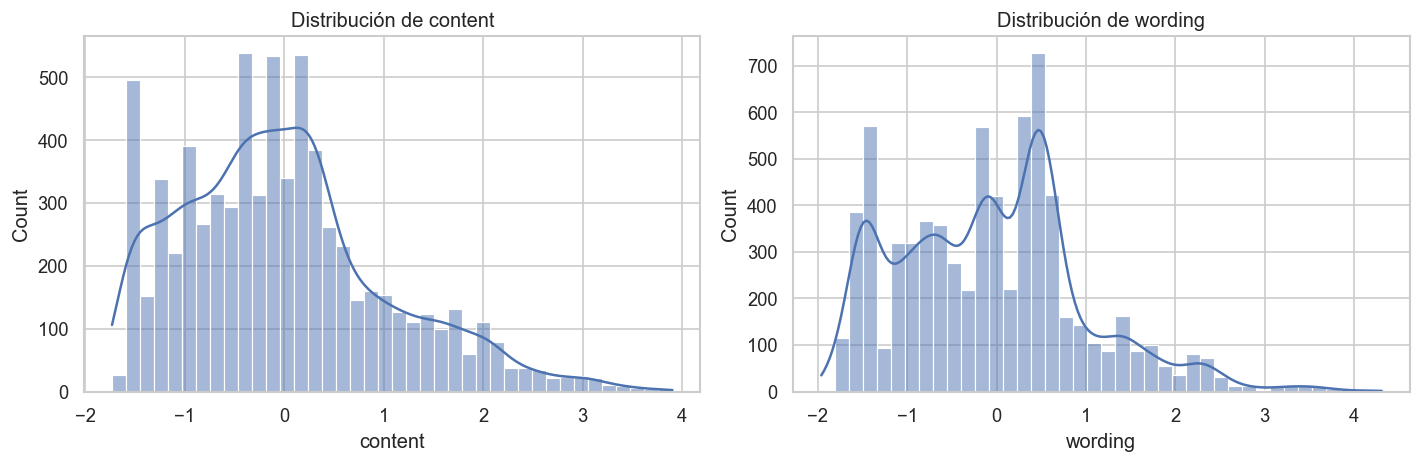
\includegraphics[width=\textwidth]{dist_targets.png}\caption{Distribución de las notas.}\end{subfigure}\hfill
\begin{subfigure}[t]{0.42\textwidth}\centering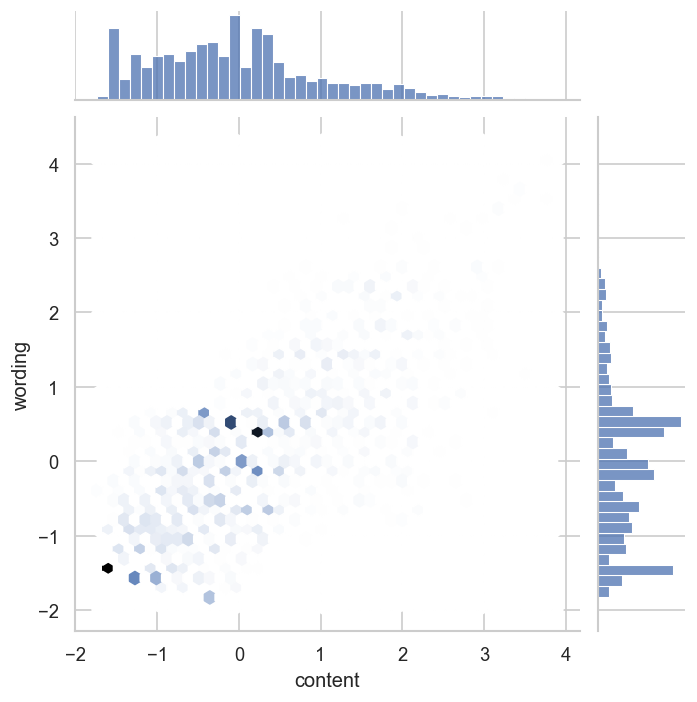
\includegraphics[width=\textwidth]{content_vs_wording.png}\caption{\emph{content} contra \emph{wording}.}\end{subfigure}
\caption{Variables objetivo.}
\label{fig:eda1}
\end{figure}

\paragraph{La longitud es la señal más fuerte.} La cantidad de palabras tiene media 74,8, mediana 58 y máximo 659; el 95\,\% de los resúmenes tiene 178 palabras o menos. La cantidad de caracteres correlaciona 0,856 con \emph{content} y 0,606 con \emph{wording}. Por quintiles de palabras, \emph{content} sube de $-1{,}09$ a $1{,}42$ y \emph{wording} de $-0{,}96$ a $0{,}85$. En cambio, la longitud del texto fuente casi no correlaciona ($-0{,}049$ con \emph{content}): importa el tamaño del resumen, no el del original. El riesgo es que un modelo se reduzca a contar palabras.

\paragraph{La diversidad léxica es un efecto del tamaño.} La razón de palabras únicas correlaciona en negativo con las dos notas ($-0{,}659$ y $-0{,}487$), pero pasa de 0,80 en los resúmenes cortos a 0,58 en los largos, porque los textos cortos tienen diversidad alta por definición. Por eso se ajusta por tamaño.

\paragraph{El solapamiento con la fuente tiene un doble efecto.} Un solapamiento medio ayuda a \emph{content}, pero uno muy alto, que equivale a copiar y pegar, baja las dos notas y sobre todo \emph{wording} (tabla~\ref{tab:quintiles}). El solapamiento de trigramas tiene mediana 0,06, pero en el percentil 95 llega a 1,0: una minoría copia frases enteras.

\begin{table}[ht]
\centering\small
\caption{Notas medias por quintil de la proporción de palabras del resumen que están en la fuente.}
\label{tab:quintiles}
\begin{tabular}{lccc}
\toprule
Quintil de solapamiento & content & wording & \makecell{solapamiento de\\trigramas} \\
\midrule
Más bajo (0 a 0,42) & $-0{,}18$ & $0{,}24$ & 0,01 \\
0,42 a 0,54 & $0{,}10$ & $0{,}27$ & 0,05 \\
0,54 a 0,64 & $0{,}17$ & $0{,}12$ & 0,11 \\
0,64 a 0,77 & $0{,}16$ & $-0{,}14$ & 0,22 \\
Más alto (0,77 a 1,0) & $-0{,}32$ & $-0{,}81$ & 0,52 \\
\bottomrule
\end{tabular}
\end{table}

\begin{figure}[ht]
\centering
\begin{subfigure}[t]{0.57\textwidth}\centering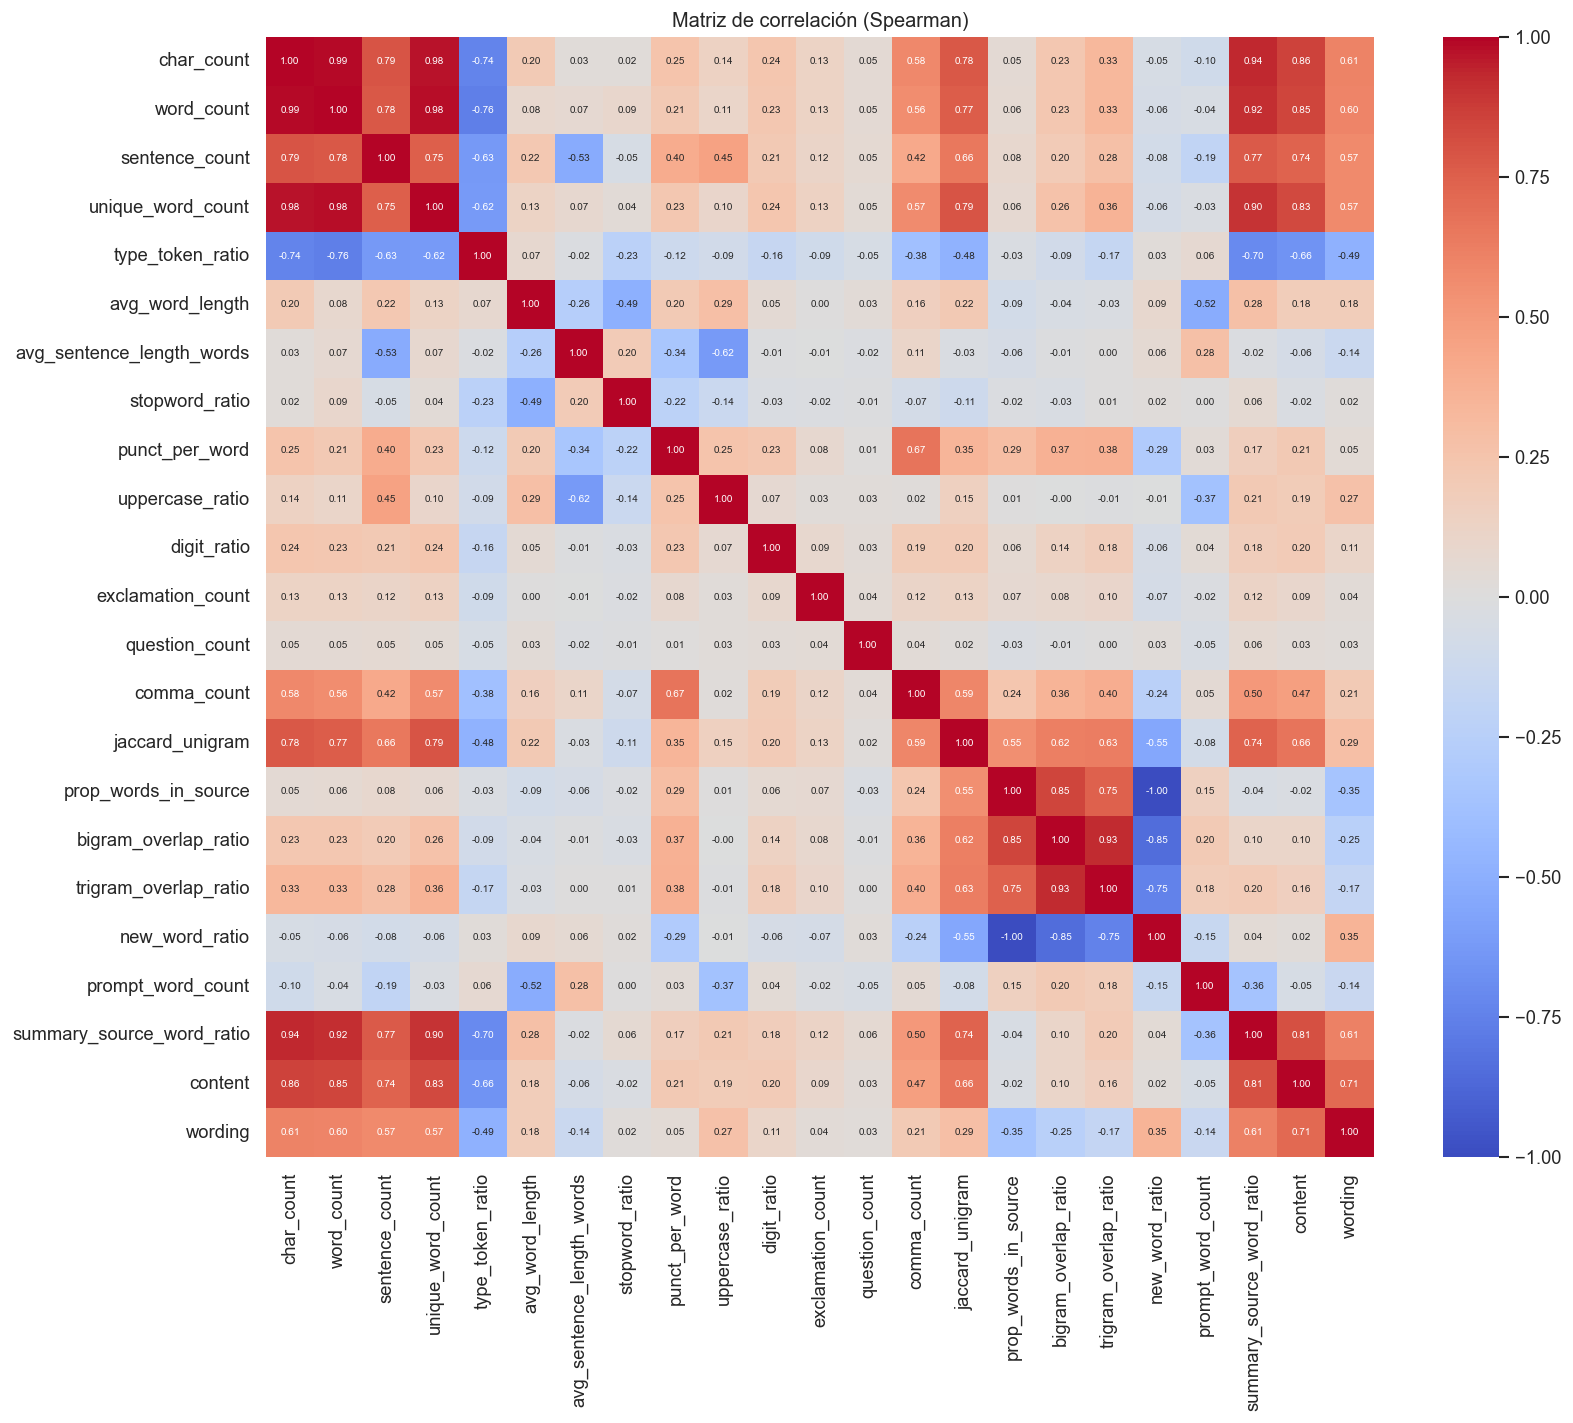
\includegraphics[width=\textwidth]{corr_heatmap.png}\caption{Correlación de Spearman entre rasgos y notas.}\end{subfigure}\hfill
\begin{subfigure}[t]{0.40\textwidth}\centering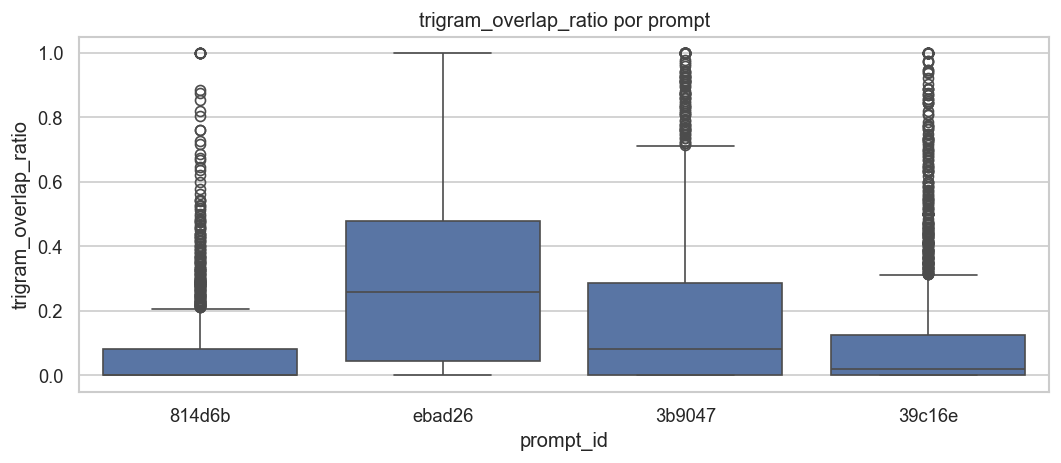
\includegraphics[width=\textwidth]{box_trigram_overlap_ratio.png}\caption{Solapamiento de trigramas por texto.}\end{subfigure}
\caption{Relación de los rasgos con las notas y diferencias entre textos.}
\label{fig:eda2}
\end{figure}

\paragraph{Hay diferencias entre textos fuente.} La nota \emph{wording} promedio es 0,52 en \emph{The Third Wave} y $-0{,}30$ en \emph{The Jungle}, casi una desviación estándar de diferencia, y \emph{On Tragedy} tiene los resúmenes más cortos y las notas más bajas (figura~\ref{fig:eda3}). Puede deberse a la dificultad del texto o al grado de los estudiantes. Esto confirma que el identificador del texto no debe usarse como variable y que la validación debe separar por texto.

\begin{figure}[ht]
\centering
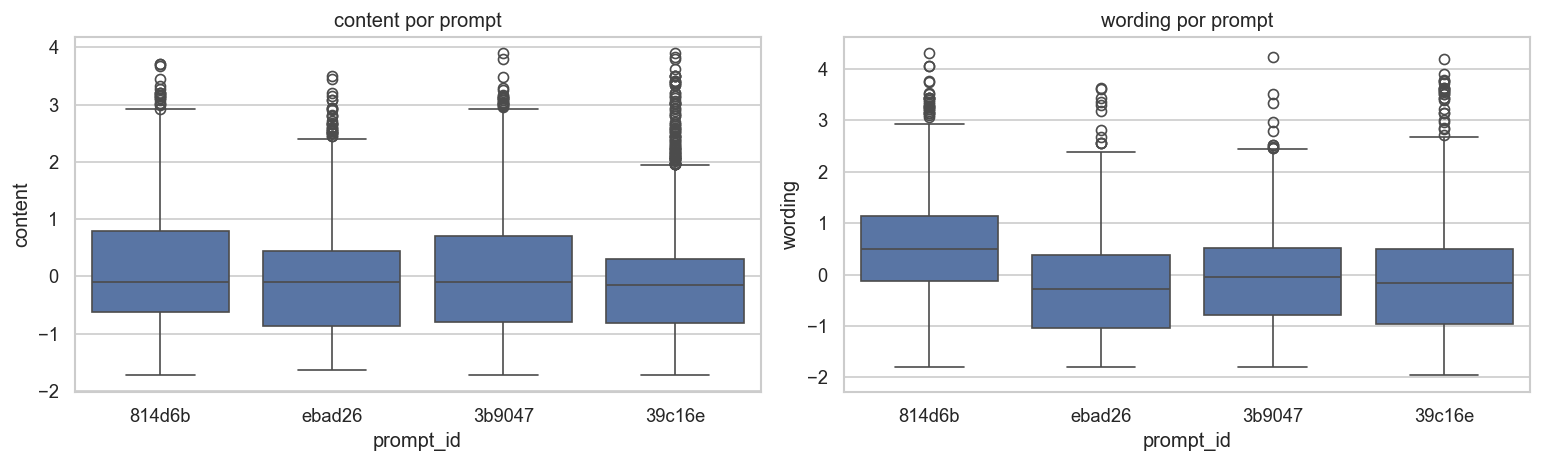
\includegraphics[width=0.85\textwidth]{box_targets_por_prompt.png}
\caption{Notas por texto fuente.}
\label{fig:eda3}
\end{figure}

\subsection{Ajuste de los parámetros de cada algoritmo}

\paragraph{Ridge.} Los rasgos se estandarizan y se elige la penalización $\alpha\in\{1,10,100,1000\}$. Con el esquema anidado se eligió $\alpha=100$ en casi todas las iteraciones, y $\alpha=1$ cuando se dejó fuera \emph{The Jungle} (tabla~\ref{tab:params}).

\paragraph{LightGBM.} Se entrena un modelo por nota. Se fijaron una tasa de aprendizaje de 0,03, un mínimo de 60 resúmenes por hoja, submuestreo de filas del 80\,\%, de columnas del 70\,\% y regularización L2 de 5, y se buscó entre 7 y 15 hojas y entre 250 y 500 árboles. Esos valores conservadores se fijaron a propósito: con cuatro textos fuente, un modelo flexible puede memorizar patrones propios de cada texto. En casi todas las iteraciones se eligieron árboles de solo 7 hojas, lo que indica que un modelo más flexible no ayuda a generalizar a un texto nuevo.

\paragraph{DeBERTa-v3.} Salida de regresión de dos neuronas sobre el promedio de las representaciones de todos los tokens, pérdida cuadrática, tasa de aprendizaje de $3\times10^{-5}$ para el modelo y $10^{-3}$ para la capa de salida, \emph{dropout} desactivado (práctica recomendada en regresión), calentamiento lineal del 10\,\% y 3 épocas fijas. La entrada es el resumen emparejado con la consigna del texto.

\begin{table}[ht]
\centering\footnotesize
\caption{Hiperparámetros elegidos en la validación interna, según el texto que se deja fuera.}
\label{tab:params}
\resizebox{\textwidth}{!}{\begin{tabular}{lcccc}
\toprule
Modelo & On Tragedy & Egyptian Social Structure & The Third Wave & The Jungle \\
\midrule
Ridge, 18 rasgos & $\alpha=10$ & $\alpha=100$ & $\alpha=100$ & $\alpha=1$ \\
Ridge, 33 rasgos & $\alpha=100$ & $\alpha=100$ & $\alpha=100$ & $\alpha=1$ \\
LightGBM, 18 rasgos & 7 hojas, 250 árb. & 7 hojas, 250 árb. & 7 hojas, 250 árb. & 7 hojas, 250 árb. \\
LightGBM, 33 rasgos & 15 hojas, 250 árb. & 7 hojas, 500 árb. & 7 hojas, 500 árb. & 7 hojas, 500 árb. \\
\bottomrule
\end{tabular}}
\end{table}


\subsection{Un hallazgo sobre la fuga de identidad del texto}
\label{sec:fuga}

En una primera versión, Ridge usaba la cantidad de palabras del texto fuente y la razón entre las palabras del resumen y las de la fuente, que el análisis exploratorio había considerado informativas. Con validación por texto, el error de Ridge en \emph{The Jungle} fue de 2,31, contra 0,50 a 0,71 en los otros tres textos (tabla~\ref{tab:fuga}). La causa es que, con solo cuatro textos fuente, la longitud del texto fuente es una constante por texto, es decir, un \emph{identificador}: el modelo lineal la usa para reconocer el texto y asigna a cada uno un desplazamiento propio. \emph{The Jungle} es el texto más largo (976 palabras) y queda fuera del rango de los otros tres, por lo que el modelo extrapola mal. La razón resumen/fuente es la longitud del resumen dividida por esa constante y arrastra el mismo problema. Se descartaron ambos rasgos. Es un caso concreto de lo que anticipó el análisis exploratorio: que el modelo no debe depender del texto, sino de rasgos del resumen.

\begin{table}[ht]
\centering\small
\caption{MCRMSE de Ridge ($\alpha=100$) por texto dejado fuera, según los rasgos usados.}
\label{tab:fuga}
\begin{tabular}{lccccc}
\toprule
Rasgos & Tragedy & Egypt & Third Wave & Jungle & Media \\
\midrule
Con longitud de la fuente y razón resumen/fuente & 0,502 & 0,710 & 0,691 & \textbf{2,308} & 1,053 \\
Sin longitud de la fuente & 0,495 & 0,710 & 0,691 & 0,517 & 0,603 \\
Sin ambos & 0,497 & 0,654 & 0,693 & 0,514 & 0,590 \\
\bottomrule
\end{tabular}
\end{table}

\subsection{Comparación de los modelos}

Las tablas~\ref{tab:modelos} y~\ref{tab:porprompt} y las figuras~\ref{fig:mcrmse}, \ref{fig:portexto}, \ref{fig:pred}, \ref{fig:longitud}, \ref{fig:imp} y~\ref{fig:tiempos} comparan los modelos. Todas las cifras son fuera de muestra: cada texto fuente se dejó fuera una vez.

\begin{table}[ht]
\centering\small
\caption{Resultados fuera de muestra (Leave-One-Prompt-Out). MCRMSE y RMSE: menor es mejor.}
\label{tab:modelos}
\resizebox{\textwidth}{!}{\begin{tabular}{lccccc}
\toprule
Modelo & \makecell{MCRMSE\\(media por texto)} & \makecell{MCRMSE\\(agrupado)} & \makecell{RMSE\\content} & \makecell{RMSE\\wording} & \makecell{Segundos\\por pliegue} \\
\midrule
Ensamble (stacking) & 0{,}518 & 0{,}511 & 0{,}433 & 0{,}588 & <0{,}1 \\
LightGBM, 33 rasgos & 0{,}524 & 0{,}518 & 0{,}448 & 0{,}587 & 0{,}5 \\
Ensamble sin DeBERTa (Ridge + LightGBM) & 0{,}545 & 0{,}538 & 0{,}460 & 0{,}616 & <0{,}1 \\
LightGBM, 18 rasgos & 0{,}546 & 0{,}540 & 0{,}466 & 0{,}615 & 0{,}2 \\
Ridge, 33 rasgos & 0{,}567 & 0{,}559 & 0{,}466 & 0{,}651 & <0{,}1 \\
Ridge, 18 rasgos & 0{,}592 & 0{,}585 & 0{,}495 & 0{,}674 & <0{,}1 \\
DeBERTa-v3 base & 0{,}608 & 0{,}610 & 0{,}484 & 0{,}737 & 495{,}4 \\
DeBERTa-v3 small & 0{,}617 & 0{,}618 & 0{,}481 & 0{,}754 & 289{,}1 \\
Línea base (solo longitud) & 0{,}724 & 0{,}712 & 0{,}559 & 0{,}865 & <0{,}1 \\
\bottomrule
\end{tabular}}
\end{table}


\begin{figure}[ht]
\centering
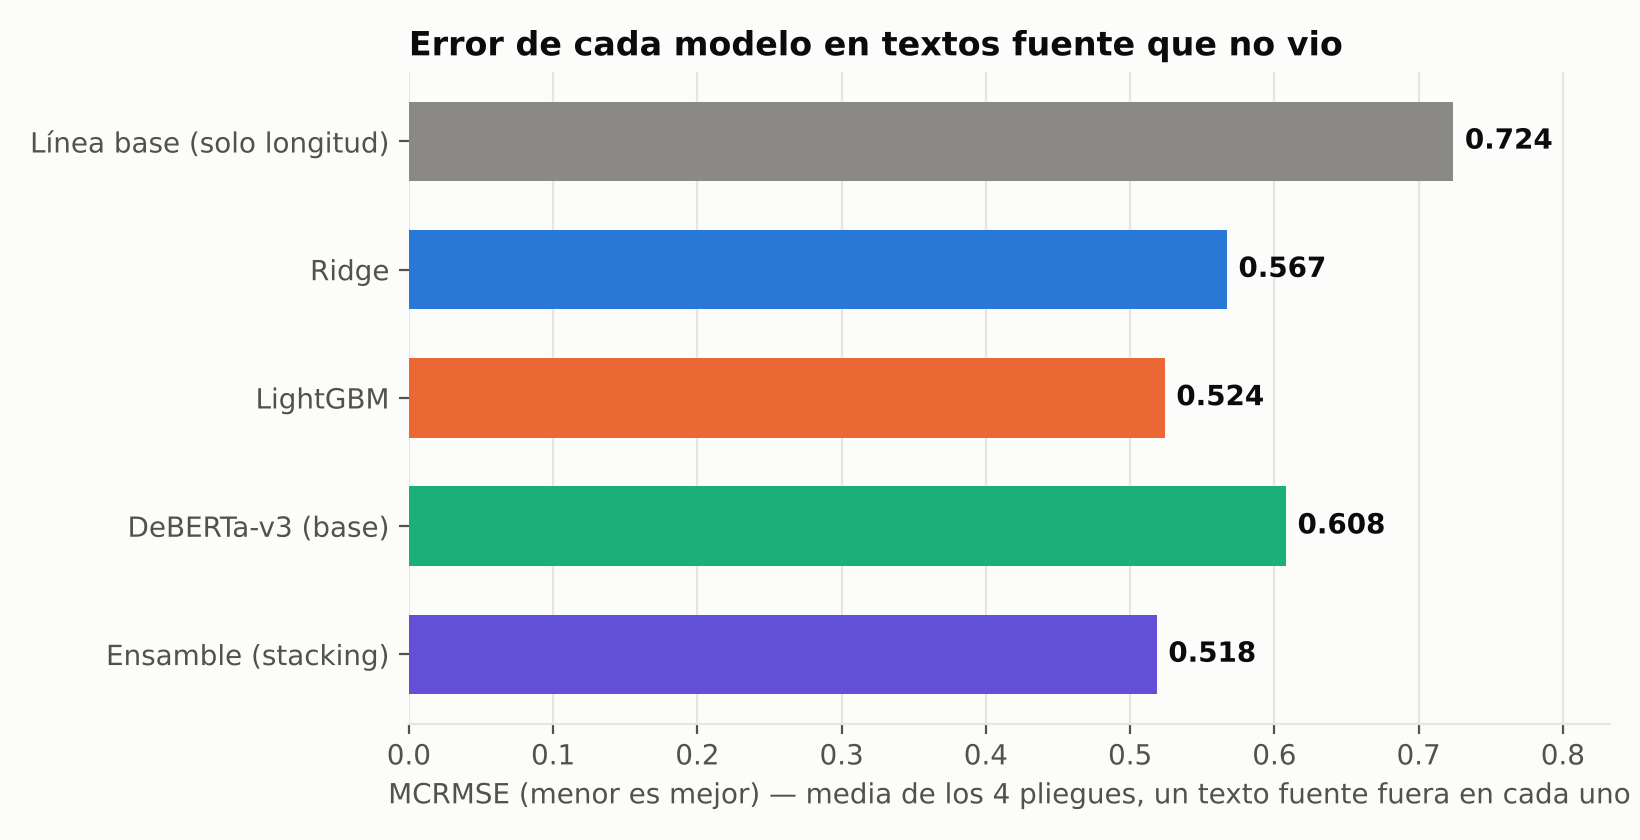
\includegraphics[width=0.85\textwidth]{fig_mcrmse_modelos.png}
\caption{Error medio de cada modelo en textos fuente que no vio (menor es mejor).}
\label{fig:mcrmse}
\end{figure}

\begin{table}[ht]
\centering\small
\caption{MCRMSE según el texto fuente que se dejó fuera de entrenamiento.}
\label{tab:porprompt}
\resizebox{\textwidth}{!}{\begin{tabular}{lcccc}
\toprule
Modelo & On Tragedy & Egyptian Social Structure & The Third Wave & The Jungle \\
\midrule
Ensamble (stacking) & 0{,}463 & 0{,}553 & 0{,}618 & 0{,}441 \\
LightGBM, 33 rasgos & 0{,}460 & 0{,}574 & 0{,}607 & 0{,}456 \\
Ensamble sin DeBERTa (Ridge + LightGBM) & 0{,}464 & 0{,}608 & 0{,}655 & 0{,}451 \\
LightGBM, 18 rasgos & 0{,}465 & 0{,}619 & 0{,}635 & 0{,}463 \\
Ridge, 33 rasgos & 0{,}486 & 0{,}586 & 0{,}654 & 0{,}542 \\
Ridge, 18 rasgos & 0{,}494 & 0{,}654 & 0{,}693 & 0{,}528 \\
DeBERTa-v3 base & 0{,}642 & 0{,}633 & 0{,}609 & 0{,}548 \\
DeBERTa-v3 small & 0{,}515 & 0{,}672 & 0{,}635 & 0{,}644 \\
Línea base (solo longitud) & 0{,}634 & 0{,}690 & 0{,}843 & 0{,}731 \\
\bottomrule
\end{tabular}}
\end{table}


\begin{figure}[ht]
\centering
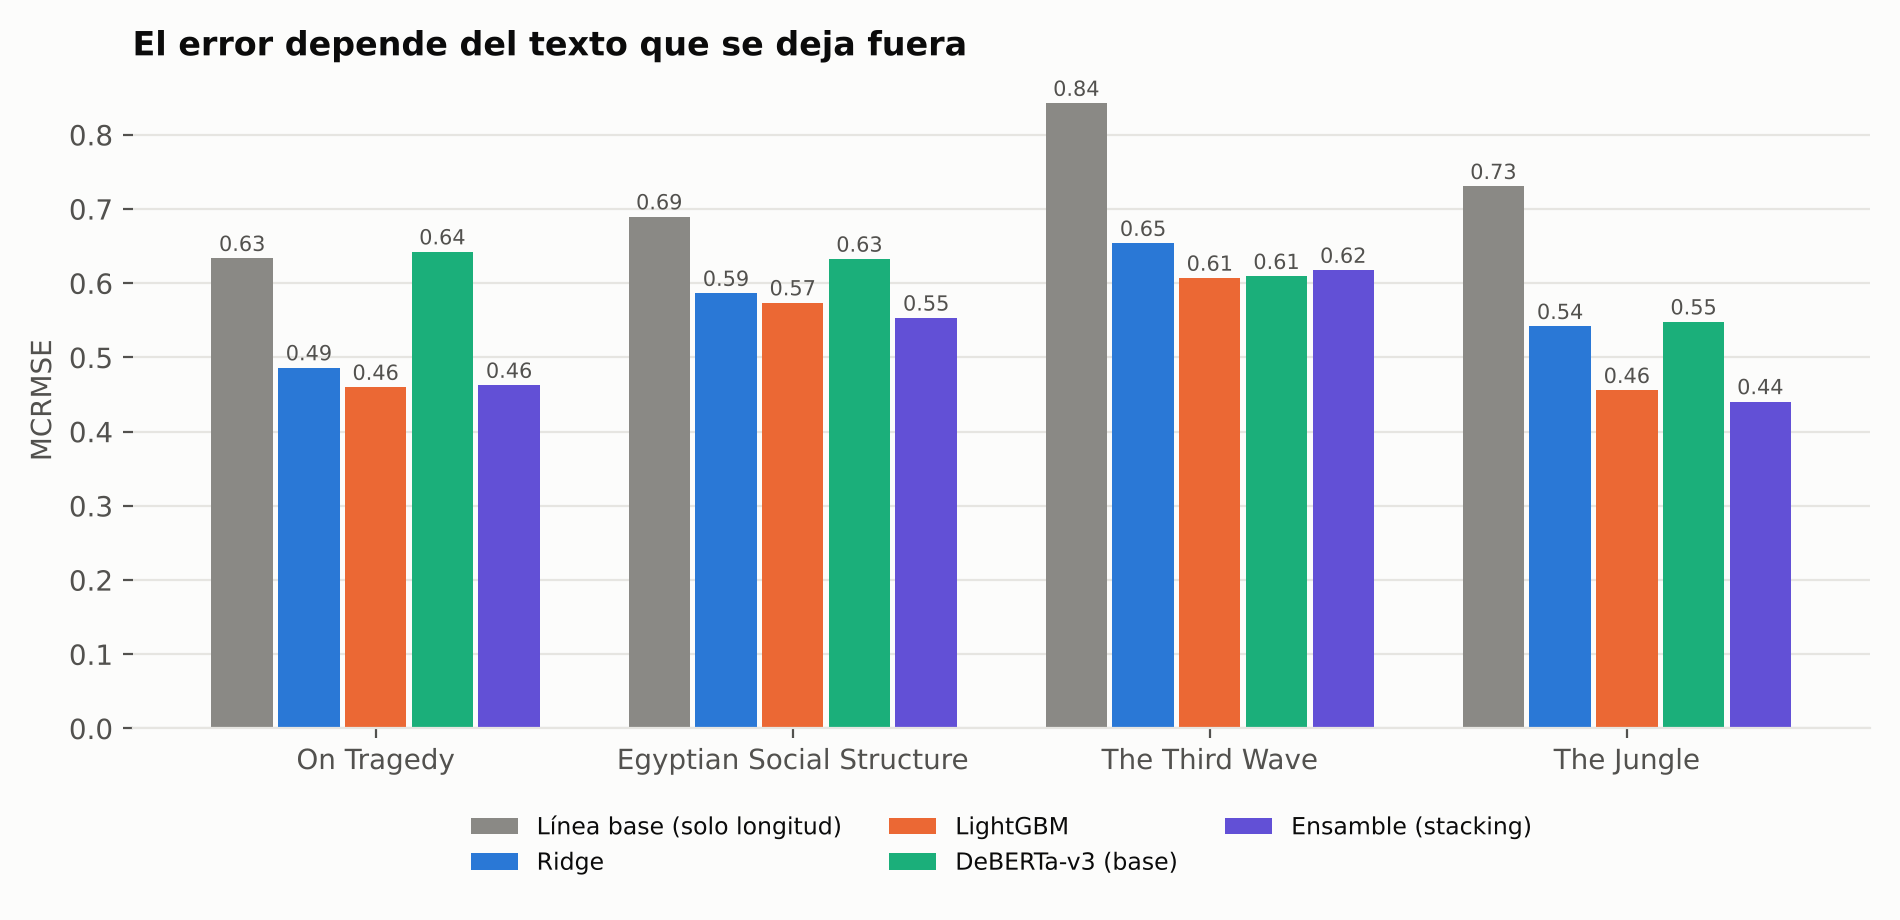
\includegraphics[width=0.9\textwidth]{fig_mcrmse_por_texto.png}
\caption{Error de cada modelo según el texto que se dejó fuera.}
\label{fig:portexto}
\end{figure}

\paragraph{Qué modelo es mejor.} El ensamble obtiene el menor error (\mcensamble), seguido de LightGBM con los 33 rasgos (\mclgbmenriquecido) y de Ridge con los 33 rasgos (\mcridgeenriquecido). DeBERTa-v3 base (\mcdebertabase) y small (\mcdebertasmall) quedan por debajo de LightGBM, aunque claramente por encima de la línea base que solo usa la longitud (\mcbaselinelongitud). Todos los modelos superan a la línea base, de modo que el contenido del texto aporta información más allá del tamaño, pero la mejora sobre ella es moderada (de \mcbaselinelongitud\ a \mcensamble) porque la longitud explica buena parte de ambas notas.

\paragraph{Efecto de los rasgos nuevos.} Pasar de 18 a 33 rasgos (legibilidad, ortografía y similitud con la fuente) reduce el error de Ridge de \mcridgebase\ a \mcridgeenriquecido\ y el de LightGBM de \mclgbmbase\ a \mclgbmenriquecido. La mejora aparece en los cuatro textos fuente para ambos modelos, salvo Ridge en el texto \texttt{ebad26}, donde empeora ligeramente (tabla~\ref{tab:porprompt}), así que no es un efecto de un solo texto. Con LightGBM la ganancia viene sobre todo de \emph{wording}.

\paragraph{DeBERTa contra LightGBM.} DeBERTa predice \emph{content} casi tan bien como LightGBM (RMSE \rcdebertabase\ contra \rclgbmenriquecido), pero es peor en \emph{wording} (\rwdebertabase\ contra \rwlgbmenriquecido). Parte de esa diferencia es un sesgo: en los resúmenes fuera de muestra DeBERTa base sobreestima \emph{wording} en promedio $0{,}36$ puntos (LightGBM, $0{,}01$), y lo hace en los cuatro textos. Es plausible que, al entrenar con tres textos, aprenda un nivel de redacción propio de ellos que no se traslada al cuarto, pero con cuatro textos no podemos comprobar esa explicación. Su entrada no incluye el texto fuente, de modo que no puede medir directamente cuánto contenido del original recoge el resumen; los rasgos de similitud sí lo hacen. Además, el modelo grande no mejora al pequeño de forma consistente: es mejor en promedio, pero el orden se invierte en \texttt{39c16e}, y con 4 pliegues y una sola semilla esa diferencia no es concluyente. En costo, el ajuste de DeBERTa base tomó cerca de 500 segundos por pliegue en GPU contra menos de un segundo de LightGBM en CPU (figura~\ref{fig:tiempos}).

\paragraph{El ensamble.} El metamodelo (Ridge con coeficientes no negativos, evaluado también fuera de muestra) da a LightGBM el mayor peso (alrededor de $0{,}55$ para \emph{content} y $0{,}62$ para \emph{wording}), a DeBERTa base un peso intermedio ($0{,}28$ y $0{,}36$) y casi nada a Ridge. El ensamble mejora a LightGBM solo en $0{,}006$ (de \mclgbmenriquecido\ a \mcensamble), una diferencia pequeña frente a la variación entre textos (de $0{,}44$ a $0{,}62$ en el ensamble) y estimada con solo cuatro pliegues; por eso no la presentamos como una ventaja establecida. La ganancia por incorporar a DeBERTa es algo más clara si se compara con el ensamble que solo usa Ridge y LightGBM (\mcensamblerasgos), pero este último es peor que LightGBM solo, lo que indica que el apilado entre modelos parecidos no ayuda. Los errores de LightGBM y DeBERTa en \emph{wording} tienen correlación de $0{,}73$, es decir, se equivocan en buena medida en los mismos resúmenes, lo que limita lo que puede aportar la combinación.

\paragraph{Por texto fuente.} El texto más difícil para el ensamble es \texttt{814d6b} (\textit{The Third Wave}), con \mcensamble\ de promedio general pero $0{,}618$ en este texto. Ahí las notas de \emph{wording} son en promedio mucho más altas ($0{,}52$) que en los otros tres textos (entre $-0{,}30$ y $-0{,}07$); LightGBM subestima esa nota en $0{,}40$, mientras que DeBERTa la sobreestima solo en $0{,}07$, y por eso es el único texto donde DeBERTa base supera a LightGBM en \emph{wording}. Un cambio de nivel entre textos, causado quizá por la dificultad del texto o por el calificador, es el principal factor de error y no se corrige con rasgos del resumen.

\paragraph{Longitud y rasgos importantes.} El error crece con la longitud del resumen para todos los modelos (figura~\ref{fig:longitud}): en el quintil de resúmenes más cortos el ensamble tiene un error de $0{,}38$ y en el de los más largos de $0{,}68$. Los rasgos que más usa LightGBM para \emph{content} son el número de caracteres ($51\,\%$ de la ganancia) y de palabras ($24\,\%$); para \emph{wording} destacan también los caracteres ($27\,\%$), el solapamiento de bigramas ($17\,\%$) y el número de oraciones ($10\,\%$) (figura~\ref{fig:imp}). La importancia mide qué usa el modelo, no por qué una nota es alta; la longitud y las notas están correlacionadas, y los modelos aprovechan esa relación.


\begin{figure}[ht]
\centering
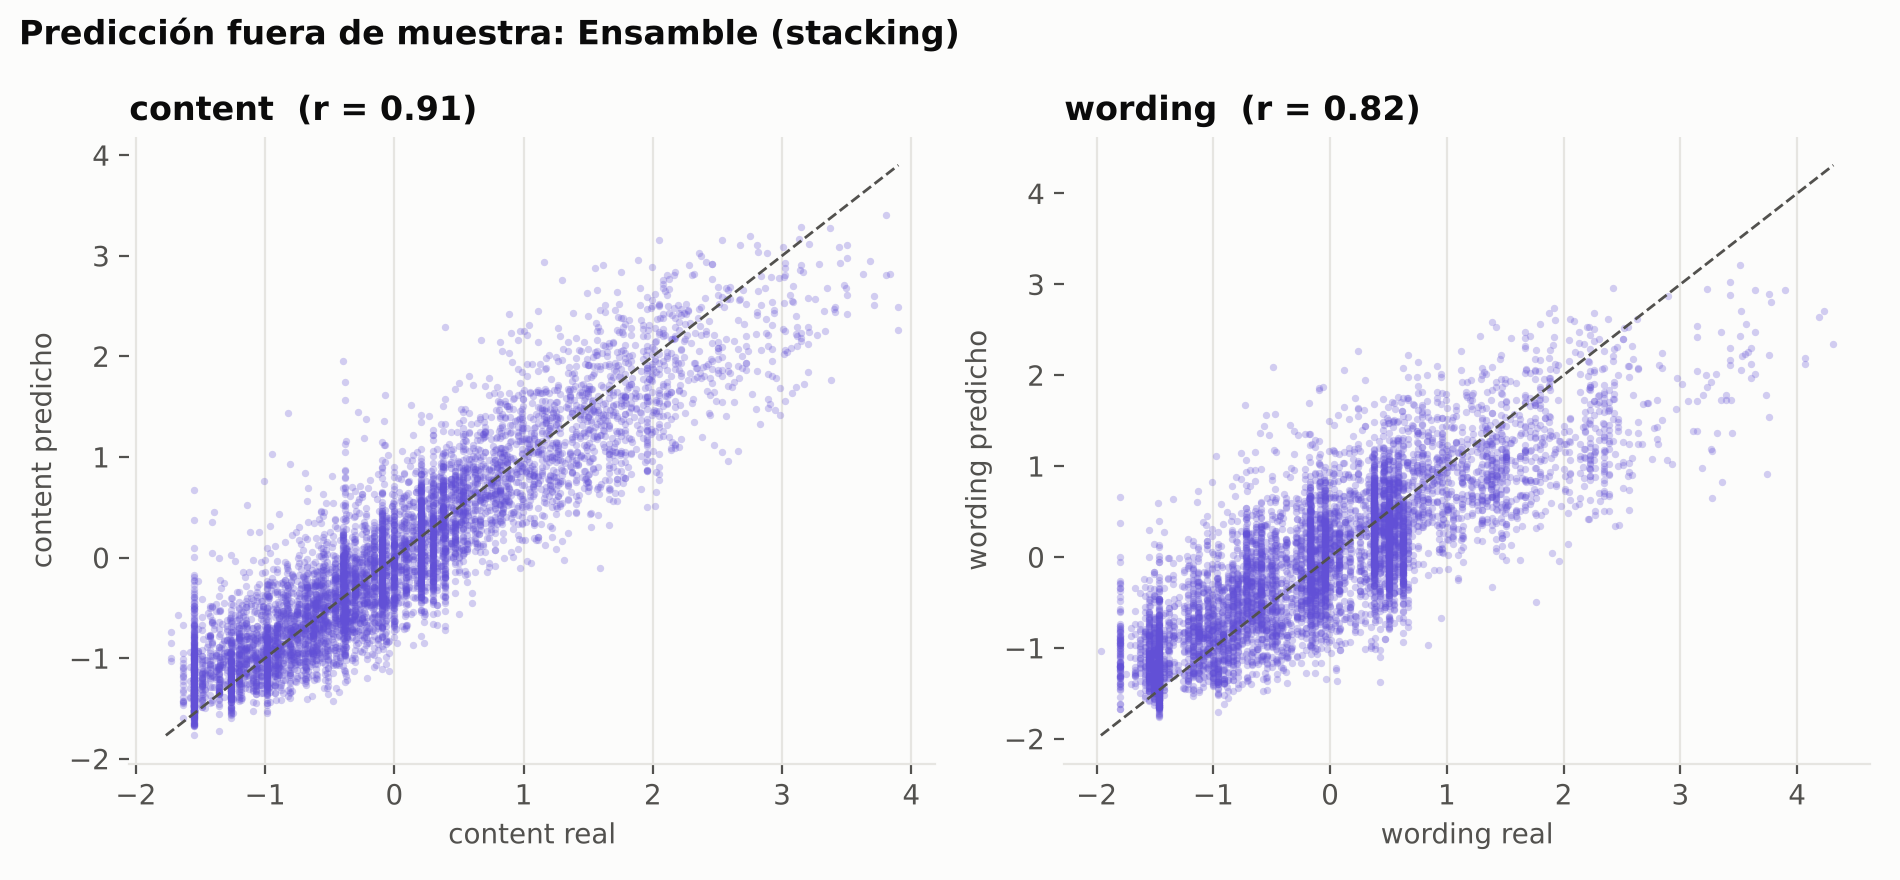
\includegraphics[width=0.95\textwidth]{fig_pred_vs_real.png}
\caption{Predicción fuera de muestra contra nota real del modelo con menor error.}
\label{fig:pred}
\end{figure}

\begin{figure}[ht]
\centering
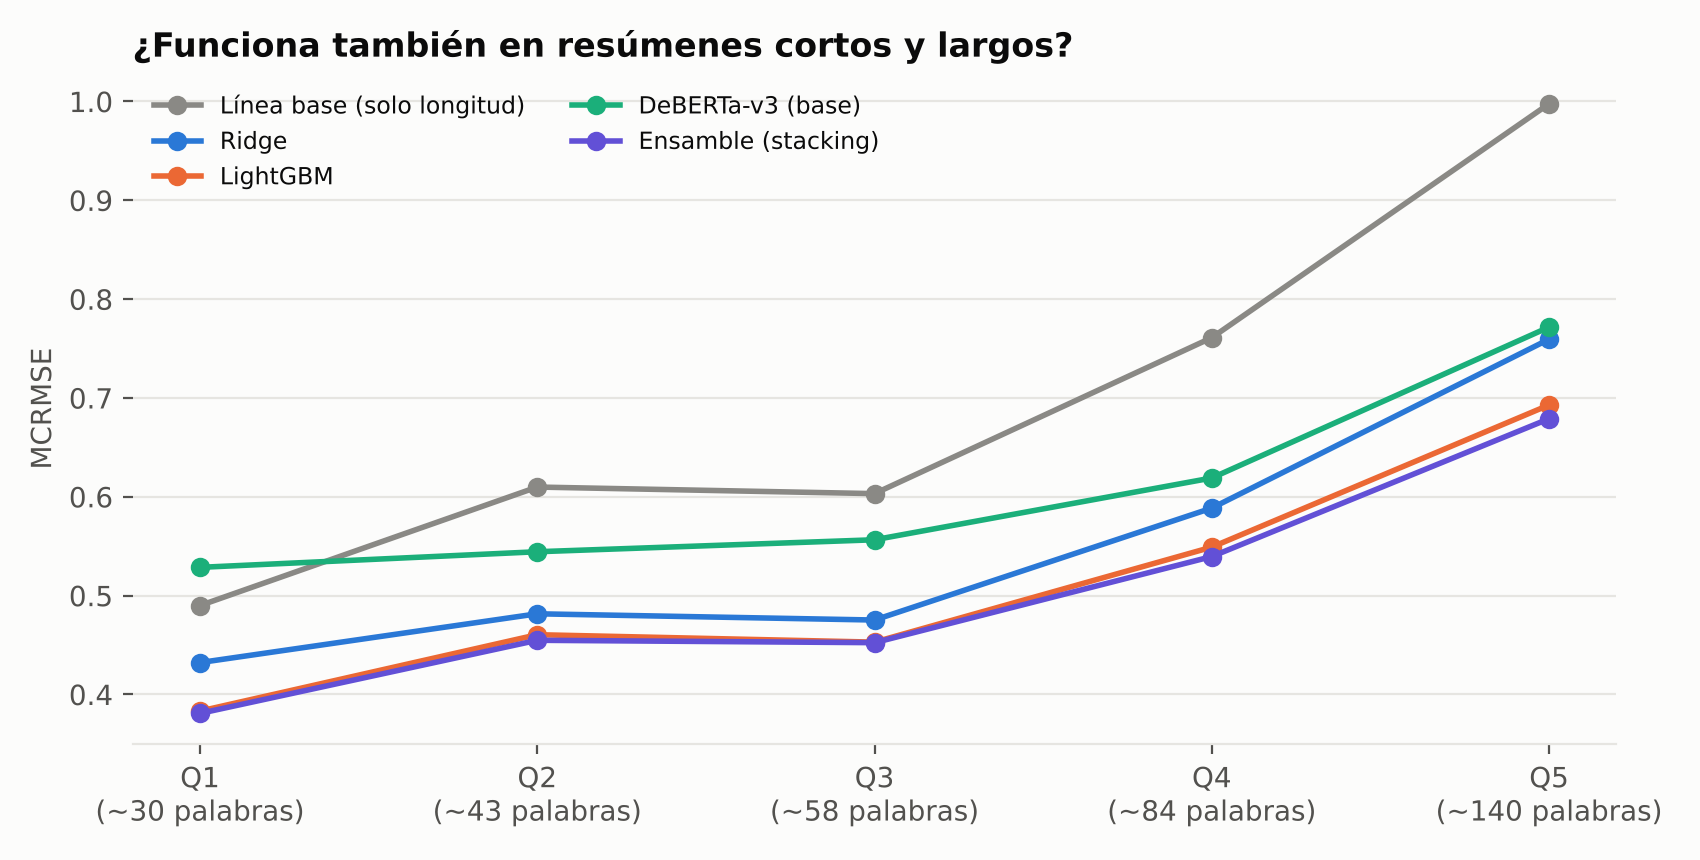
\includegraphics[width=0.85\textwidth]{fig_error_por_longitud.png}
\caption{Error según la longitud del resumen (quintiles de cantidad de palabras).}
\label{fig:longitud}
\end{figure}

\begin{figure}[ht]
\centering
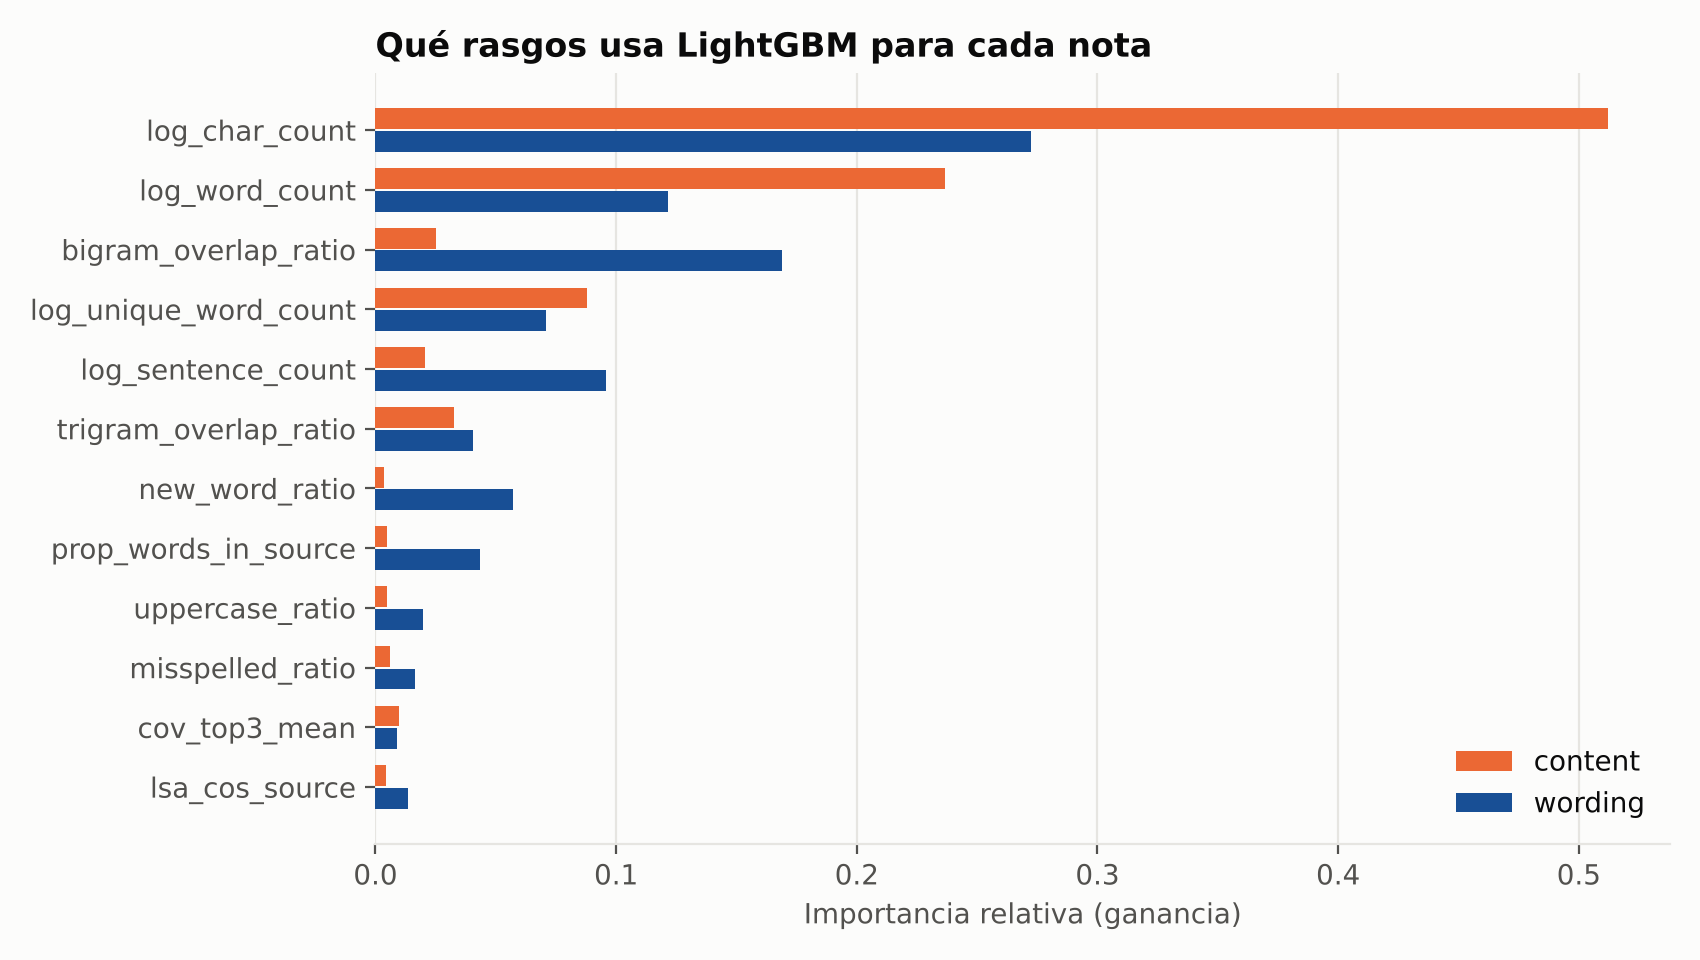
\includegraphics[width=0.85\textwidth]{fig_importancia_lightgbm.png}
\caption{Rasgos que más usa LightGBM para cada nota.}
\label{fig:imp}
\end{figure}

\begin{figure}[ht]
\centering
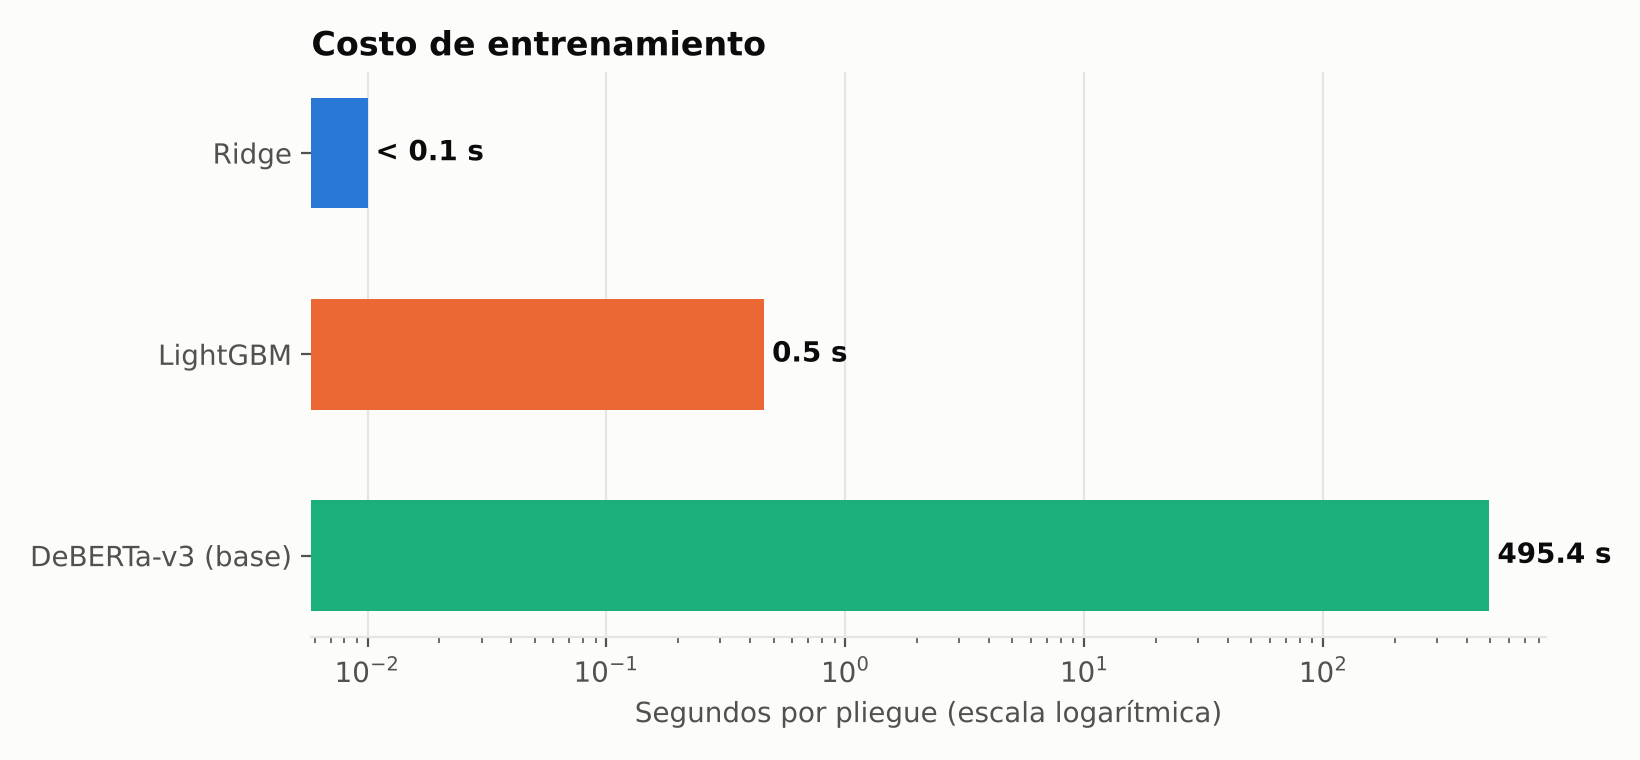
\includegraphics[width=0.8\textwidth]{fig_tiempos.png}
\caption{Tiempo de ajuste por pliegue (escala logarítmica).}
\label{fig:tiempos}
\end{figure}


\subsection{Aplicación para probar los modelos}

Se construyó una aplicación web con \textbf{Streamlit} y \textbf{Plotly}. Streamlit permite escribir la interfaz en Python y reutilizar directamente el código de limpieza, rasgos y modelos del proyecto, de modo que el preprocesamiento ocurre dentro de la aplicación y pasa inadvertido para el usuario. Plotly produce gráficas interactivas (información al pasar el cursor, acercamiento y selección de series) que funcionan en el navegador. La aplicación se ejecuta con \texttt{streamlit run app/app.py}.

La aplicación tiene tres pestañas y una barra lateral de controles (figuras~\ref{fig:app1}, \ref{fig:app2} y \ref{fig:app3}):
\begin{itemize}[nosep]
\item \textbf{Calificar un resumen}. El usuario elige uno de los cuatro textos del curso o pega un texto fuente propio, escribe o pega un resumen (o carga uno real de ejemplo, con sus notas reales de referencia) y pulsa \emph{Calificar}. Se muestran las notas \emph{content} y \emph{wording} de cada modelo, una gráfica que las compara, avisos cuando el resumen es muy corto, muy largo o se parece demasiado a la fuente, y la posición del resumen respecto de los 7\,165 del entrenamiento.
\item \textbf{Explorar los datos}. Variables del conjunto después de la limpieza, incluidas las que usan los modelos. El usuario elige una variable y una nota y ve su distribución, su relación con la nota (con el promedio por tramos), su correlación con todas las demás variables y su estadística descriptiva, con la opción de separar por texto fuente.
\item \textbf{Rendimiento de los modelos}. MCRMSE global y por texto, gráfica de predicho contra real, error según la longitud del resumen e importancia de los rasgos de LightGBM. Todas las cifras son fuera de muestra.
\item \textbf{Barra lateral}. Permite ver el resultado de \textbf{cada algoritmo por separado o de todos} a la vez y \textbf{ocultar} la pestaña de rendimiento con un interruptor.
\end{itemize}

\paragraph{Selección de colores.} La interfaz usa un fondo neutro cálido y texto casi negro, y reserva el color para los datos. Cada modelo tiene un color fijo en toda la aplicación y en las figuras del informe (azul para Ridge, naranja para LightGBM, verde azulado para DeBERTa y violeta para el ensamble), mientras que la línea base es gris porque es una referencia y no un candidato. Los colores siguen al modelo, no a su posición en el ranking, así que un filtro no cambia el color de los demás. Se escogieron tonos de luminosidad parecida y buena separación entre vecinos, y se verificó con una validación numérica que sean distinguibles también para personas con daltonismo (diferencia de color mínima de 9,2 entre modelos adyacentes con simulación de deuteranopía, medida en OKLab$\times$100). Como el verde azulado tiene poco contraste con el fondo claro, todas las barras llevan su valor escrito y la tabla de resultados está disponible. La pareja \emph{content}/\emph{wording} se distingue por relleno liso y rayado y no por color, para no competir con la identidad del modelo.

\begin{figure}[ht]
\centering
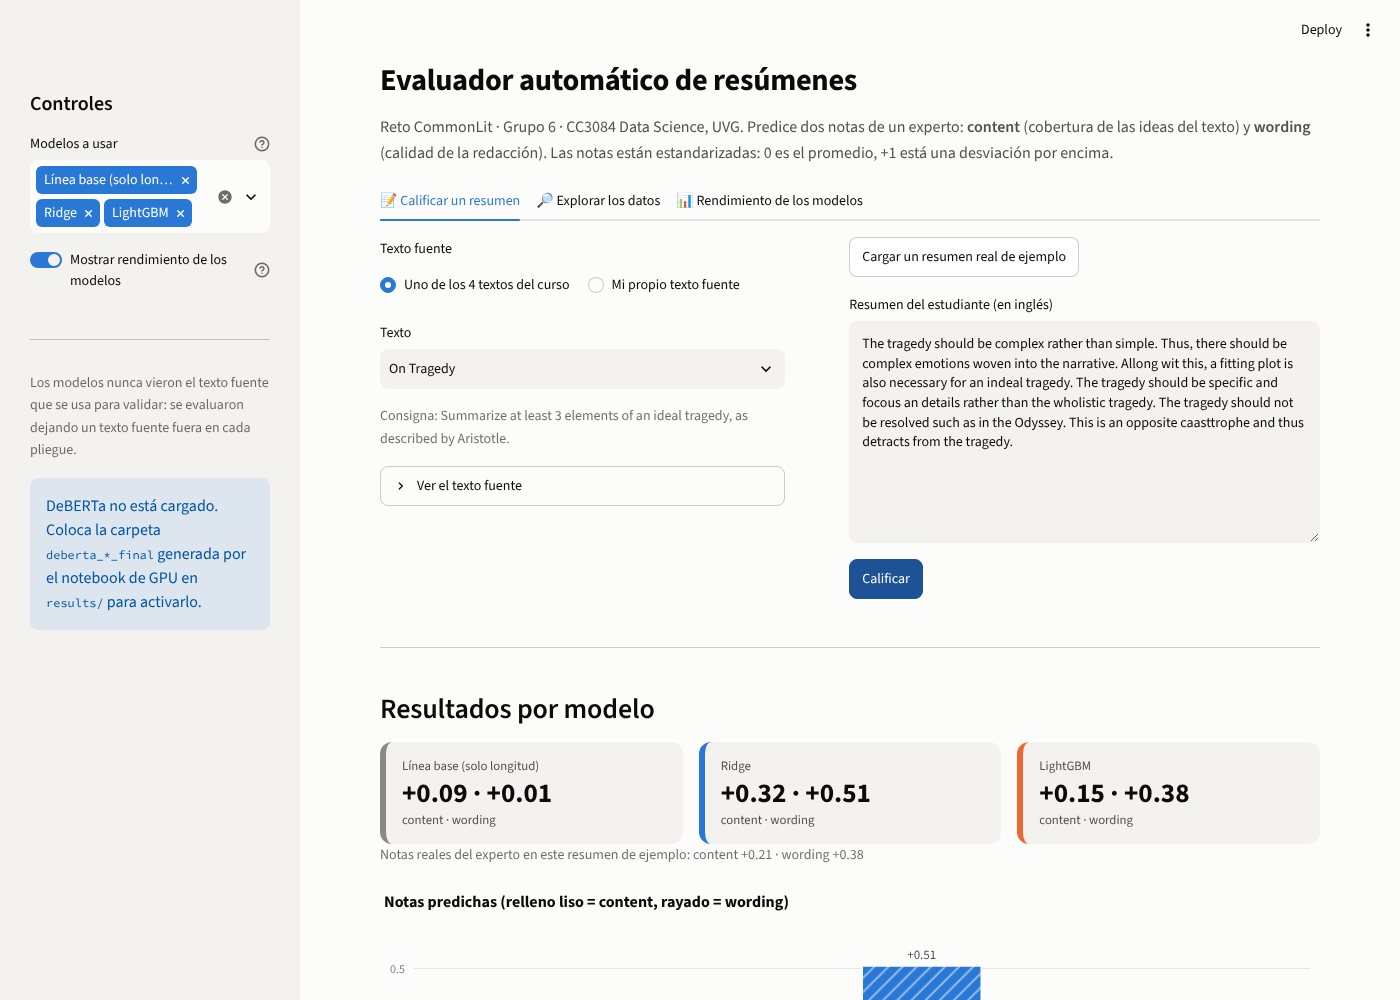
\includegraphics[width=0.95\textwidth]{app/app_calificar.png}
\caption{Pestaña \emph{Calificar un resumen}: notas predichas por cada modelo para un resumen de ejemplo.}
\label{fig:app1}
\end{figure}

\begin{figure}[ht]
\centering
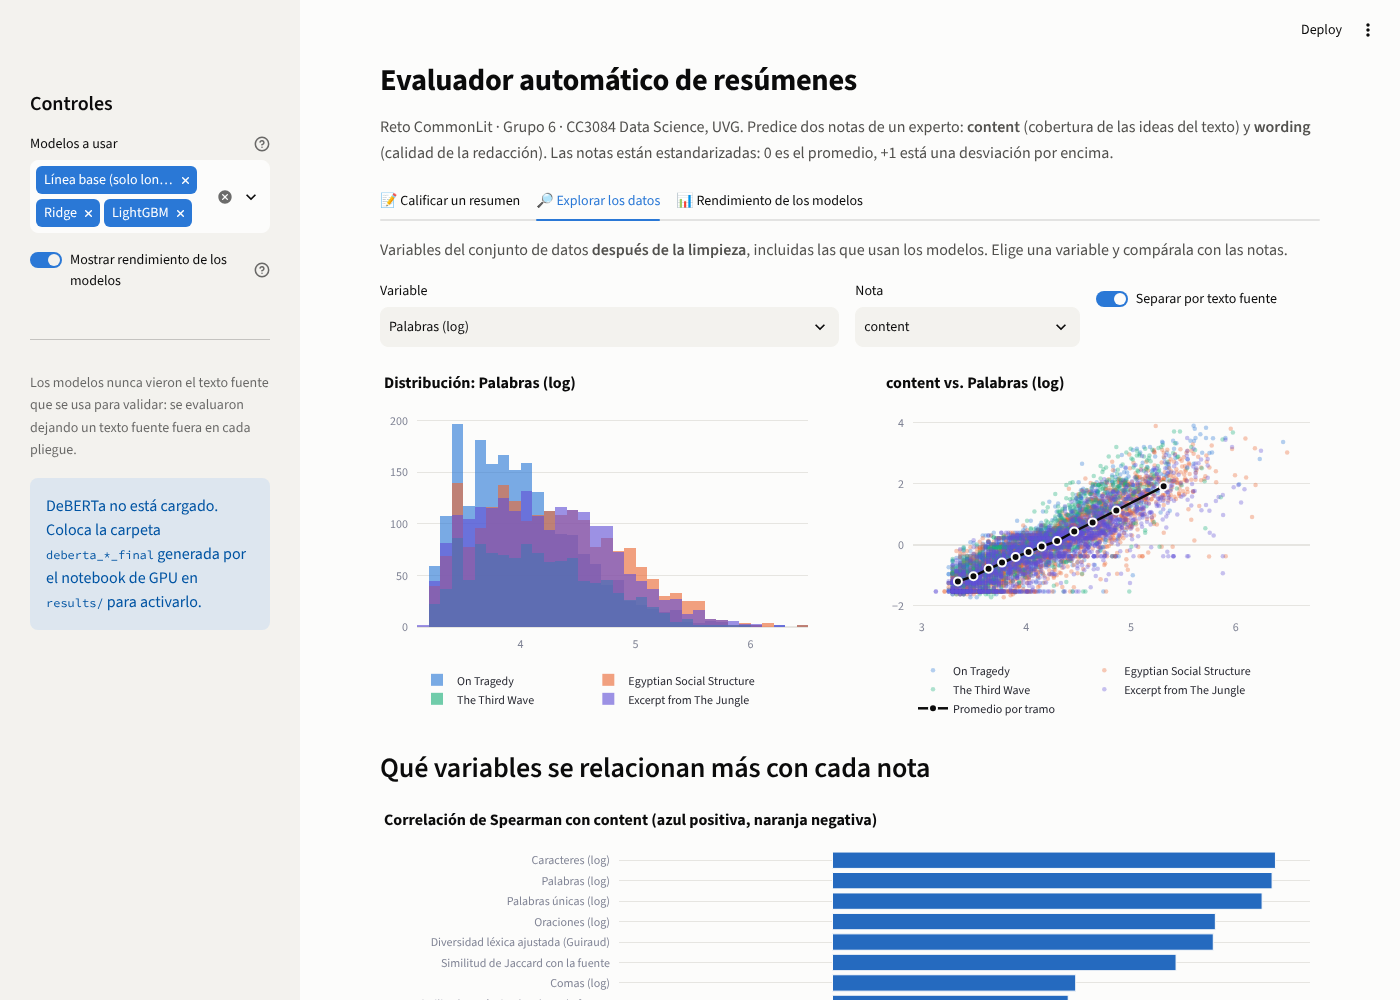
\includegraphics[width=0.95\textwidth]{app/app_explorar.png}
\caption{Pestaña \emph{Explorar los datos}.}
\label{fig:app2}
\end{figure}

\begin{figure}[ht]
\centering
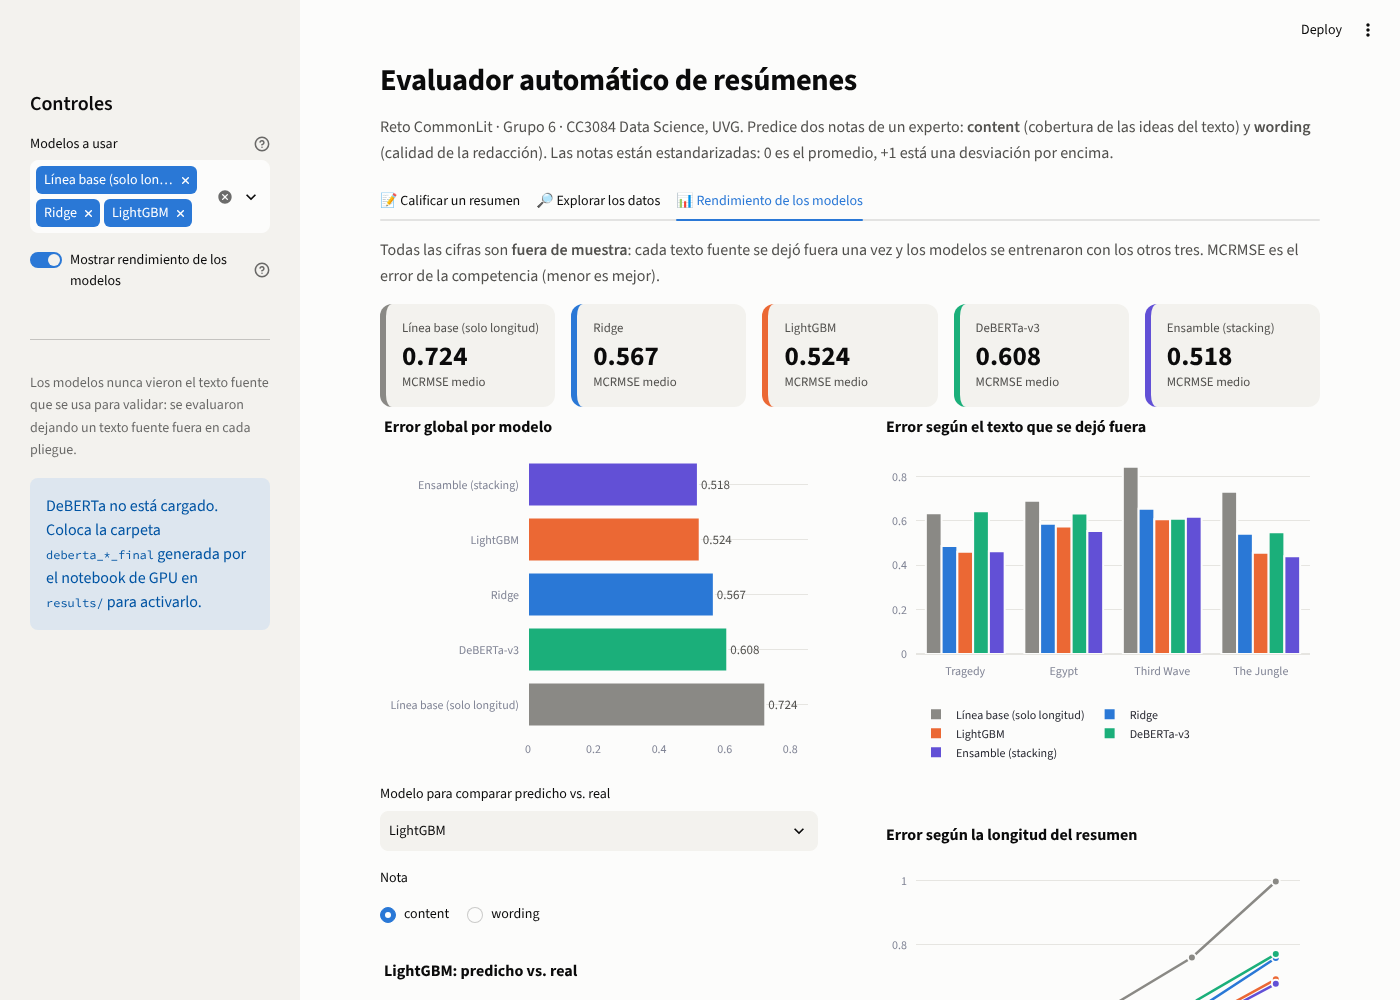
\includegraphics[width=0.95\textwidth]{app/app_rendimiento.png}
\caption{Pestaña \emph{Rendimiento de los modelos}, que se puede ocultar desde la barra lateral.}
\label{fig:app3}
\end{figure}

\section{Conclusiones}

\begin{itemize}[nosep]
\item \textbf{Modelos y comparación.} Se compararon una línea base de longitud, Ridge, LightGBM y DeBERTa-v3 (small y base) con validación que deja fuera un texto fuente completo, para medir la generalización a textos nuevos. El menor error fue el del ensamble (MCRMSE \mcensamble), seguido de LightGBM con 33 rasgos (\mclgbmenriquecido); DeBERTa quedó en \mcdebertabase\ (base) y la línea base en \mcbaselinelongitud.
\item \textbf{Rasgos.} Los rasgos de legibilidad, ortografía y similitud con la fuente bajaron el error de Ridge y de LightGBM en la mayoría de los textos. Por el contrario, las variables constantes dentro de un texto fuente identifican al texto y arruinan la generalización, por lo que se retiraron.
\item \textbf{DeBERTa.} No superó a LightGBM con rasgos en este conjunto, pues sobreestima \emph{wording} en textos nuevos. Su valor está en el ensamble, donde recibe un peso apreciable, aunque la mejora sobre LightGBM (alrededor de $0{,}006$) es pequeña y no se puede distinguir del azar con cuatro pliegues.
\item \textbf{Aplicación.} La aplicación permite calificar un resumen, explorar las variables y ver el rendimiento de cada algoritmo por separado o en conjunto, con gráficos interactivos que se pueden ocultar.
\end{itemize}

\paragraph{Limitaciones.} Solo hay cuatro textos fuente, así que cada estimación depende de cuatro pliegues y de una semilla; las diferencias de unas pocas centésimas no son concluyentes. La entrada de DeBERTa no incluye el texto fuente. La similitud semántica usa TF-IDF y LSA, no embeddings de oraciones, y la legibilidad y la ortografía usan implementaciones propias. Las notas dependen de los calificadores, y el desfase de \emph{wording} en el texto \texttt{814d6b} sugiere que parte del error no es explicable con el resumen. El conjunto de prueba oculto no estuvo disponible, así que no se reporta una cifra sobre él.

\paragraph{Trabajo futuro.} Probar DeBERTa con el texto fuente como entrada, repetir con varias semillas, usar embeddings de oraciones para la similitud, y calibrar el nivel de cada texto con unos pocos ejemplos calificados.

\begin{thebibliography}{99}

\bibitem[Attali y Burstein(2006)]{attali2006}
Attali, Y., y Burstein, J. (2006). Automated essay scoring with e-rater V.2. \textit{The Journal of Technology, Learning, and Assessment, 4}(3). \url{https://ejournals.bc.edu/index.php/jtla/article/view/1650}

\bibitem[Bojanowski et~al.(2017)]{bojanowski2017}
Bojanowski, P., Grave, E., Joulin, A., y Mikolov, T. (2017). Enriching word vectors with subword information. \textit{Transactions of the Association for Computational Linguistics, 5}, 135--146. \url{https://doi.org/10.1162/tacl_a_00051}

\bibitem[Breiman(2001)]{breiman2001}
Breiman, L. (2001). Random forests. \textit{Machine Learning, 45}(1), 5--32. \url{https://doi.org/10.1023/A:1010933404324}

\bibitem[Burrows et~al.(2015)]{burrows2015}
Burrows, S., Gurevych, I., y Stein, B. (2015). The eras and trends of automatic short answer grading. \textit{International Journal of Artificial Intelligence in Education, 25}(1), 60--117. \url{https://doi.org/10.1007/s40593-014-0026-8}

\bibitem[Chen y Guestrin(2016)]{chen2016}
Chen, T., y Guestrin, C. (2016). XGBoost: A scalable tree boosting system. En \textit{Proceedings of the 22nd ACM SIGKDD International Conference on Knowledge Discovery and Data Mining} (pp. 785--794). ACM. \url{https://doi.org/10.1145/2939672.2939785}

\bibitem[Cortes y Vapnik(1995)]{cortes1995}
Cortes, C., y Vapnik, V. (1995). Support-vector networks. \textit{Machine Learning, 20}(3), 273--297. \url{https://doi.org/10.1007/BF00994018}

\bibitem[Crossley et~al.(2016)]{crossley2016}
Crossley, S. A., Kyle, K., y McNamara, D. S. (2016). The tool for the automatic analysis of text cohesion (TAACO): Automatic assessment of local, global, and text cohesion. \textit{Behavior Research Methods, 48}(4), 1227--1237. \url{https://doi.org/10.3758/s13428-015-0651-7}

\bibitem[Devlin et~al.(2019)]{devlin2019}
Devlin, J., Chang, M.-W., Lee, K., y Toutanova, K. (2019). BERT: Pre-training of deep bidirectional transformers for language understanding. En \textit{Proceedings of the 2019 Conference of the North American Chapter of the Association for Computational Linguistics: Human Language Technologies} (pp. 4171--4186). Association for Computational Linguistics. \url{https://doi.org/10.18653/v1/N19-1423}

\bibitem[Franzke et~al.(2005)]{franzke2005}
Franzke, M., Kintsch, E., Caccamise, D., Johnson, N., y Dooley, S. (2005). Summary Street®: Computer support for comprehension and writing. \textit{Journal of Educational Computing Research, 33}(1), 53--80. \url{https://doi.org/10.2190/DH8F-QJWM-J457-FQVB}

\bibitem[Friedman(2001)]{friedman2001}
Friedman, J. H. (2001). Greedy function approximation: A gradient boosting machine. \textit{The Annals of Statistics, 29}(5), 1189--1232. \url{https://doi.org/10.1214/aos/1013203451}

\bibitem[He et~al.(2021)]{he2021}
He, P., Liu, X., Gao, J., y Chen, W. (2021). DeBERTa: Decoding-enhanced BERT with disentangled attention. En \textit{International Conference on Learning Representations}. \url{https://arxiv.org/abs/2006.03654}

\bibitem[He et~al.(2023)]{he2023}
He, P., Gao, J., y Chen, W. (2023). \textit{DeBERTaV3: Improving DeBERTa using ELECTRA-style pre-training with gradient-disentangled embedding sharing} [Preprint]. arXiv. \url{https://arxiv.org/abs/2111.09543}

\bibitem[Hochreiter y Schmidhuber(1997)]{hochreiter1997}
Hochreiter, S., y Schmidhuber, J. (1997). Long short-term memory. \textit{Neural Computation, 9}(8), 1735--1780. \url{https://doi.org/10.1162/neco.1997.9.8.1735}

\bibitem[Hoerl y Kennard(1970)]{hoerl1970}
Hoerl, A. E., y Kennard, R. W. (1970). Ridge regression: Biased estimation for nonorthogonal problems. \textit{Technometrics, 12}(1), 55--67. \url{https://doi.org/10.2307/1267351}

\bibitem[Hussein et~al.(2019)]{hussein2019}
Hussein, M. A., Hassan, H., y Nassef, M. (2019). Automated language essay scoring systems: A literature review. \textit{PeerJ Computer Science, 5}, e208. \url{https://doi.org/10.7717/peerj-cs.208}

\bibitem[Ke et~al.(2017)]{ke2017}
Ke, G., Meng, Q., Finley, T., Wang, T., Chen, W., Ma, W., Ye, Q., y Liu, T.-Y. (2017). LightGBM: A highly efficient gradient boosting decision tree. En \textit{Advances in Neural Information Processing Systems 30}. \url{https://papers.nips.cc/paper/6907-lightgbm-a-highly-efficient-gradient-boosting-decision-tree}

\bibitem[Kintsch et~al.(2000)]{kintsch2000}
Kintsch, E., Steinhart, D., Stahl, G., LSA Research Group, Matthews, C., y Lamb, R. (2000). Developing summarization skills through the use of LSA-based feedback. \textit{Interactive Learning Environments, 8}(2), 87--109. \url{https://doi.org/10.1076/1049-4820(200008)8:2;1-B;FT087}

\bibitem[Kumar y Boulanger(2020)]{kumar2020}
Kumar, V., y Boulanger, D. (2020). Explainable automated essay scoring: Deep learning really has pedagogical value. \textit{Frontiers in Education, 5}, 572367. \url{https://doi.org/10.3389/feduc.2020.572367}

\bibitem[Kyle et~al.(2018)]{kyle2018}
Kyle, K., Crossley, S., y Berger, C. (2018). The tool for the automatic analysis of lexical sophistication (TAALES): Version 2.0. \textit{Behavior Research Methods, 50}(3), 1030--1046. \url{https://doi.org/10.3758/s13428-017-0924-4}

\bibitem[Landauer et~al.(1998)]{landauer1998}
Landauer, T. K., Foltz, P. W., y Laham, D. (1998). An introduction to latent semantic analysis. \textit{Discourse Processes, 25}(2--3), 259--284. \url{https://doi.org/10.1080/01638539809545028}

\bibitem[Ludwig et~al.(2021)]{ludwig2021}
Ludwig, S., Mayer, C., Hansen, C., Eilers, K., y Brandt, S. (2021). Automated essay scoring using transformer models. \textit{Psych, 3}(4), 897--915. \url{https://doi.org/10.3390/psych3040056}

\bibitem[Mizumoto y Eguchi(2023)]{mizumoto2023}
Mizumoto, A., y Eguchi, M. (2023). Exploring the potential of using an AI language model for automated essay scoring. \textit{Research Methods in Applied Linguistics, 2}(2), 100050. \url{https://doi.org/10.1016/j.rmal.2023.100050}

\bibitem[Pedregosa et~al.(2011)]{pedregosa2011}
Pedregosa, F., Varoquaux, G., Gramfort, A., Michel, V., Thirion, B., Grisel, O., Blondel, M., Prettenhofer, P., Weiss, R., Dubourg, V., Vanderplas, J., Passos, A., Cournapeau, D., Brucher, M., Perrot, M., y Duchesnay, E. (2011). Scikit-learn: Machine learning in Python. \textit{Journal of Machine Learning Research, 12}, 2825--2830. \url{https://jmlr.org/papers/v12/pedregosa11a.html}

\bibitem[Ramesh y Sanampudi(2022)]{ramesh2022}
Ramesh, D., y Sanampudi, S. K. (2022). An automated essay scoring systems: A systematic literature review. \textit{Artificial Intelligence Review, 55}(3), 2495--2527. \url{https://doi.org/10.1007/s10462-021-10068-2}

\bibitem[Reimers y Gurevych(2019)]{reimers2019}
Reimers, N., y Gurevych, I. (2019). Sentence-BERT: Sentence embeddings using Siamese BERT-networks. En \textit{Proceedings of the 2019 Conference on Empirical Methods in Natural Language Processing and the 9th International Joint Conference on Natural Language Processing} (pp. 3982--3992). Association for Computational Linguistics. \url{https://doi.org/10.18653/v1/D19-1410}

\bibitem[Salton y Buckley(1988)]{salton1988}
Salton, G., y Buckley, C. (1988). Term-weighting approaches in automatic text retrieval. \textit{Information Processing \& Management, 24}(5), 513--523. \url{https://doi.org/10.1016/0306-4573(88)90021-0}

\bibitem[Shwartz-Ziv y Armon(2022)]{shwartz2022}
Shwartz-Ziv, R., y Armon, A. (2022). Tabular data: Deep learning is not all you need. \textit{Information Fusion, 81}, 84--90. \url{https://doi.org/10.1016/j.inffus.2021.11.011}

\bibitem[Smola y Sch{\"o}lkopf(2004)]{smola2004}
Smola, A. J., y Sch{\"o}lkopf, B. (2004). A tutorial on support vector regression. \textit{Statistics and Computing, 14}(3), 199--222. \url{https://doi.org/10.1023/B:STCO.0000035301.49549.88}

\bibitem[Taghipour y Ng(2016)]{taghipour2016}
Taghipour, K., y Ng, H. T. (2016). A neural approach to automated essay scoring. En \textit{Proceedings of the 2016 Conference on Empirical Methods in Natural Language Processing} (pp. 1882--1891). Association for Computational Linguistics. \url{https://doi.org/10.18653/v1/D16-1193}

\bibitem[Uto(2021)]{uto2021}
Uto, M. (2021). A review of deep-neural automated essay scoring models. \textit{Behaviormetrika, 48}(2), 459--484. \url{https://doi.org/10.1007/s41237-021-00142-y}

\bibitem[Wade-Stein y Kintsch(2004)]{wade2004}
Wade-Stein, D., y Kintsch, E. (2004). Summary Street: Interactive computer support for writing. \textit{Cognition and Instruction, 22}(3), 333--362. \url{https://doi.org/10.1207/s1532690xci2203_3}

\bibitem[Williamson et~al.(2012)]{williamson2012}
Williamson, D. M., Xi, X., y Breyer, F. J. (2012). A framework for evaluation and use of automated scoring. \textit{Educational Measurement: Issues and Practice, 31}(1), 2--13. \url{https://doi.org/10.1111/j.1745-3992.2011.00223.x}

\bibitem[Wolpert(1992)]{wolpert1992}
Wolpert, D. H. (1992). Stacked generalization. \textit{Neural Networks, 5}(2), 241--259. \url{https://doi.org/10.1016/S0893-6080(05)80023-1}

\bibitem[Xue et~al.(2021)]{xue2021}
Xue, J., Tang, X., y Zheng, L. (2021). A hierarchical BERT-based transfer learning approach for multi-dimensional essay scoring. \textit{IEEE Access, 9}, 125403--125415. \url{https://doi.org/10.1109/ACCESS.2021.3110683}


\bibitem[Flesch(1948)]{flesch1948}
Flesch, R. (1948). A new readability yardstick. \textit{Journal of Applied Psychology, 32}(3), 221--233. \url{https://doi.org/10.1037/h0057532}

\bibitem[Hirschberg y Manning(2015)]{hirschberg2015}
Hirschberg, J., y Manning, C. D. (2015). Advances in natural language processing. \textit{Science, 349}(6245), 261--266. \url{https://doi.org/10.1126/science.aaa8685}

\bibitem[McCarthy y Jarvis(2010)]{mccarthy2010}
McCarthy, P. M., y Jarvis, S. (2010). MTLD, vocd-D, and HD-D: A validation study of sophisticated approaches to lexical diversity assessment. \textit{Behavior Research Methods, 42}(2), 381--392. \url{https://doi.org/10.3758/BRM.42.2.381}

\bibitem[Roberts et~al.(2017)]{roberts2017}
Roberts, D. R., Bahn, V., Ciuti, S., Boyce, M. S., Elith, J., Guillera-Arroita, G., Hauenstein, S., Lahoz-Monfort, J. J., Schröder, B., Thuiller, W., Warton, D. I., Wintle, B. A., Hartig, F., y Dormann, C. F. (2017). Cross-validation strategies for data with temporal, spatial, hierarchical, or phylogenetic structure. \textit{Ecography, 40}(8), 913--929. \url{https://doi.org/10.1111/ecog.02881}

\bibitem[Uysal y Gunal(2014)]{uysal2014}
Uysal, A. K., y Gunal, S. (2014). The impact of preprocessing on text classification. \textit{Information Processing \& Management, 50}(1), 104--112. \url{https://doi.org/10.1016/j.ipm.2013.08.006}

\end{thebibliography}

\end{document}
